\newpage
\section{Additional Graphs}
\label{appendix:roc}

\subsubsection{ROC Curves Compared to Other Methods}

% short, abs, edge
\begin{figure}[H]
    \centering
    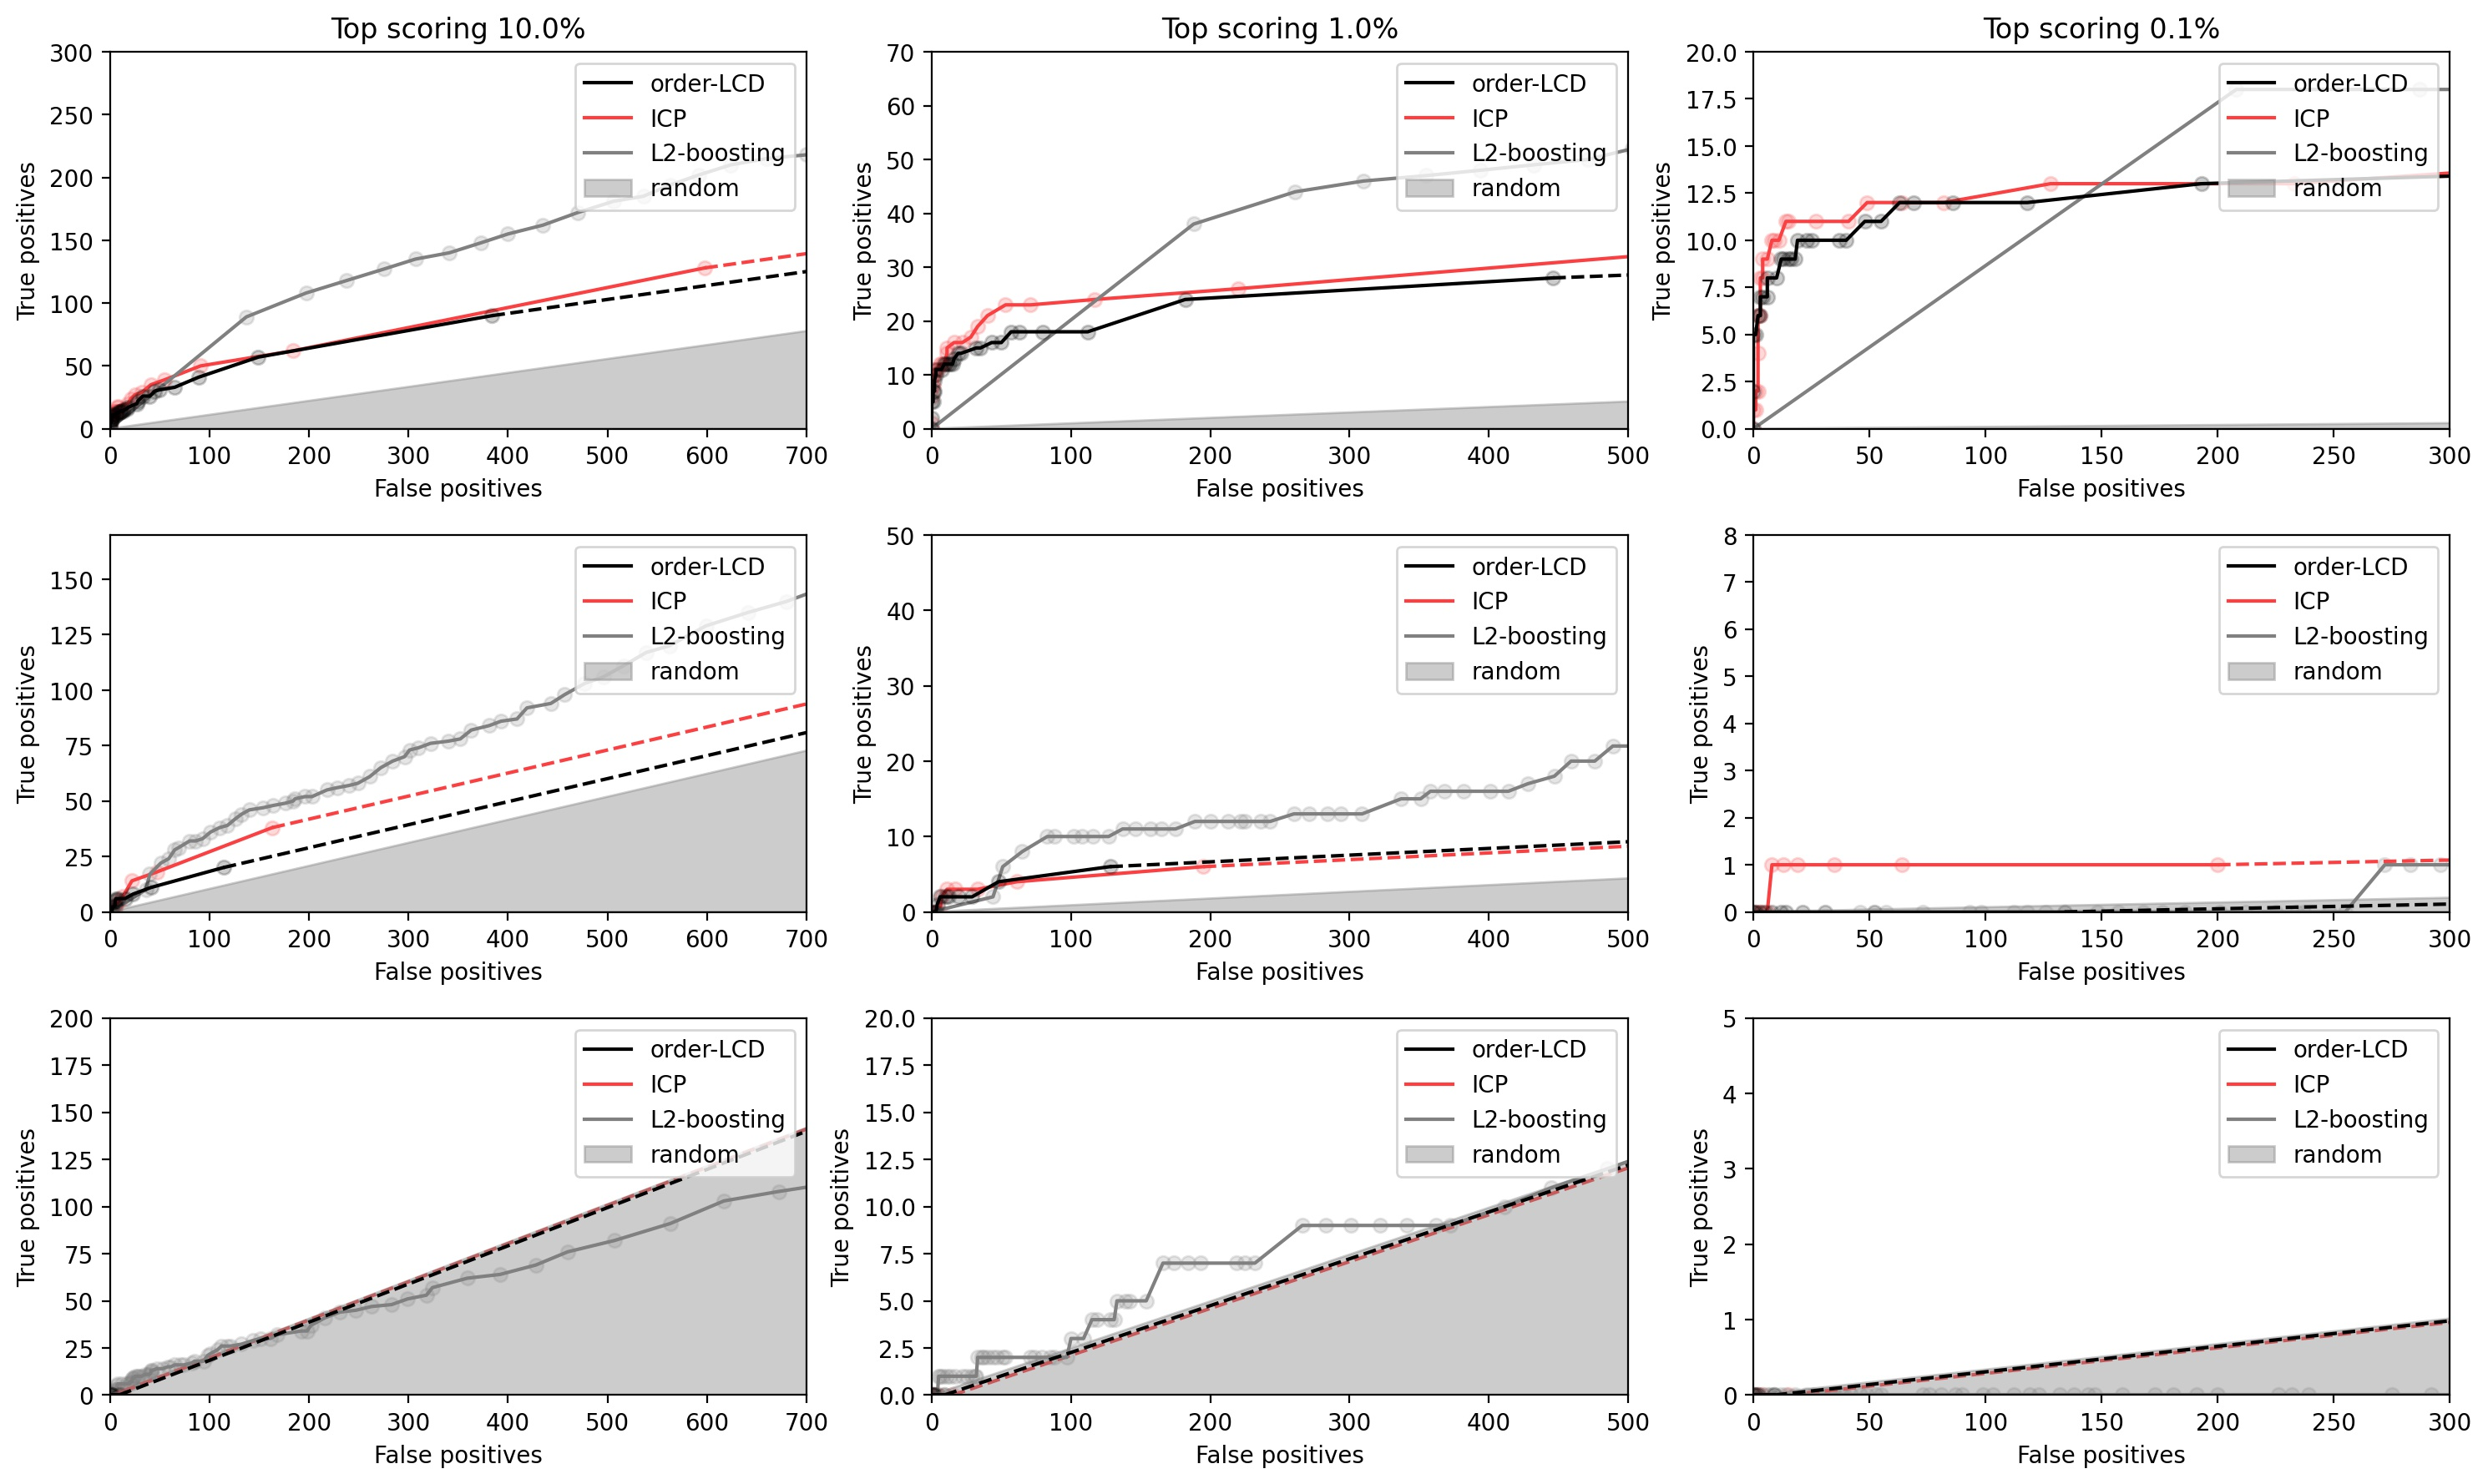
\includegraphics[width=.9\textwidth]{BROC_abs_dis_met.jpg}
    \caption{ROC curves of order-based LCD compared to other methods. \textbf{Discrete predictions} are evaluated on the \textbf{absolute ground-truth}. Columns use different ground-truth thresholds, rows different subsets of the relations that are evaluated. A dashed line indicates that a method resorts to random guessing.}
\end{figure}
% short, abs, score
\begin{figure}[H]
    \centering
    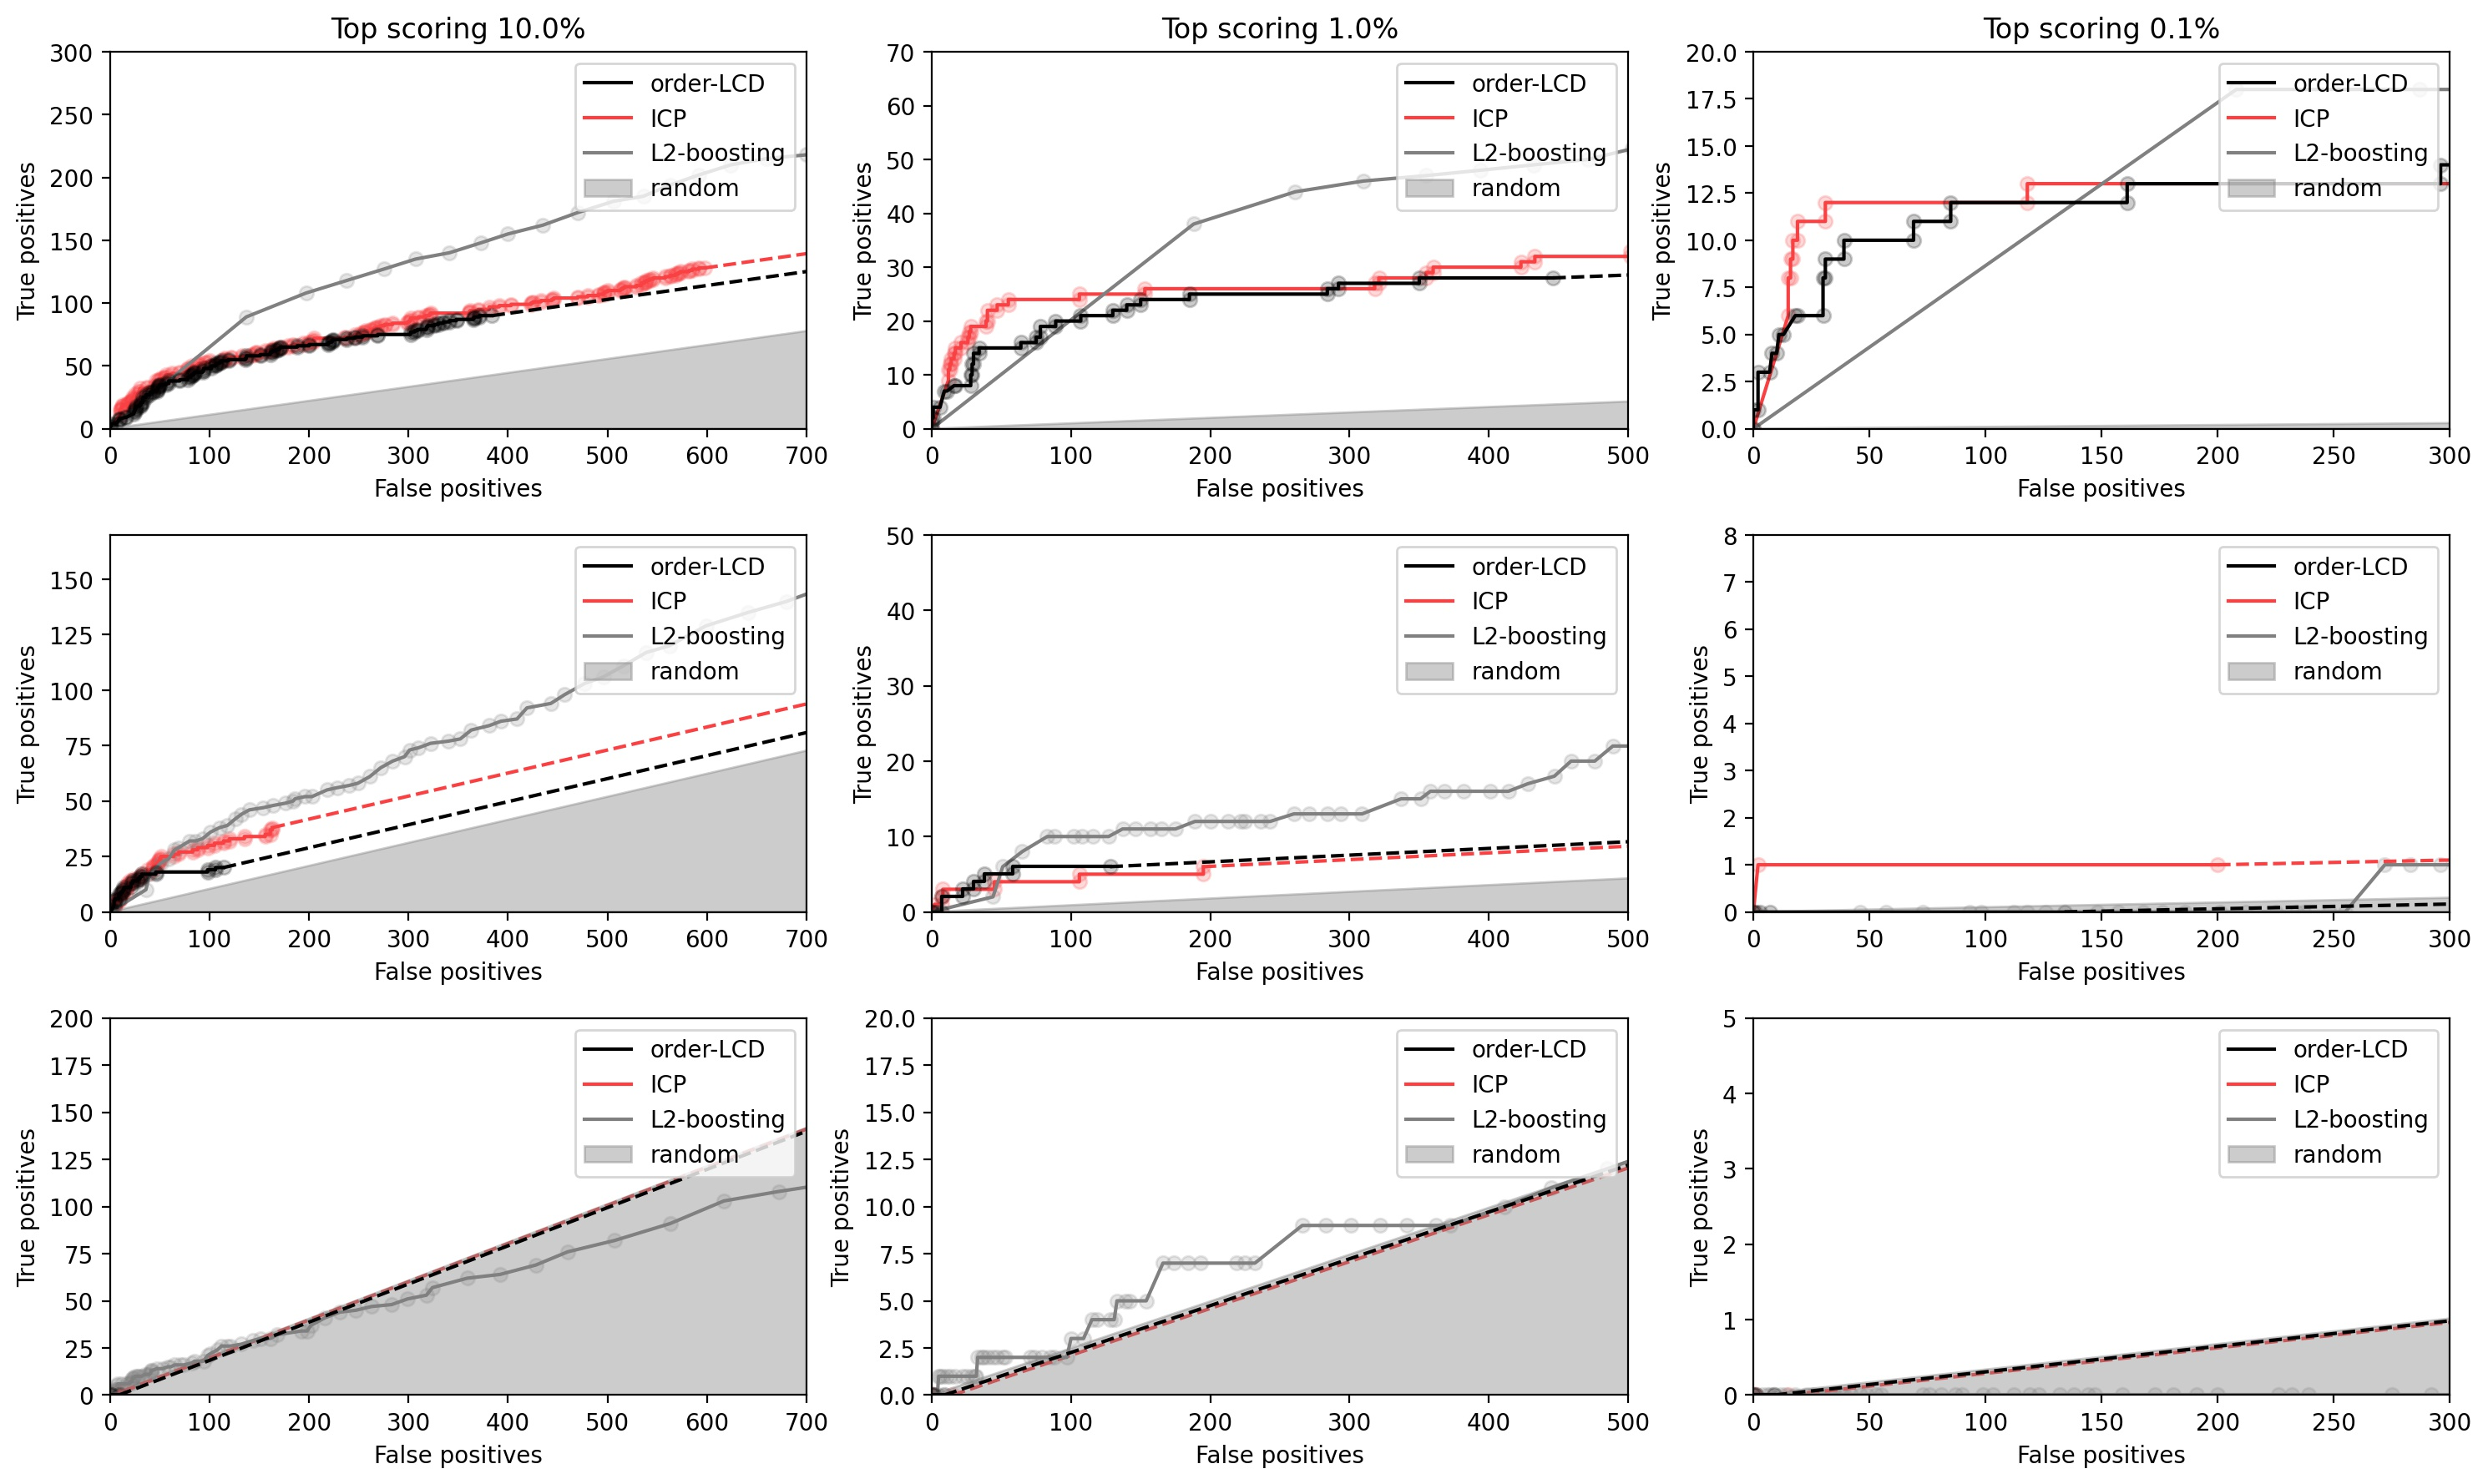
\includegraphics[width=.9\textwidth]{BROC_abs_con_met.jpg}
    \caption{ROC curves of order-based LCD compared to other methods. \textbf{Continuous predictions} are evaluated on the \textbf{absolute ground-truth}. Columns use different ground-truth thresholds, rows different subsets of the relations that are evaluated. A dashed line indicates that a method resorts to random guessing.}
\end{figure}
% short, norm, edge
\begin{figure}[H]
    \centering
    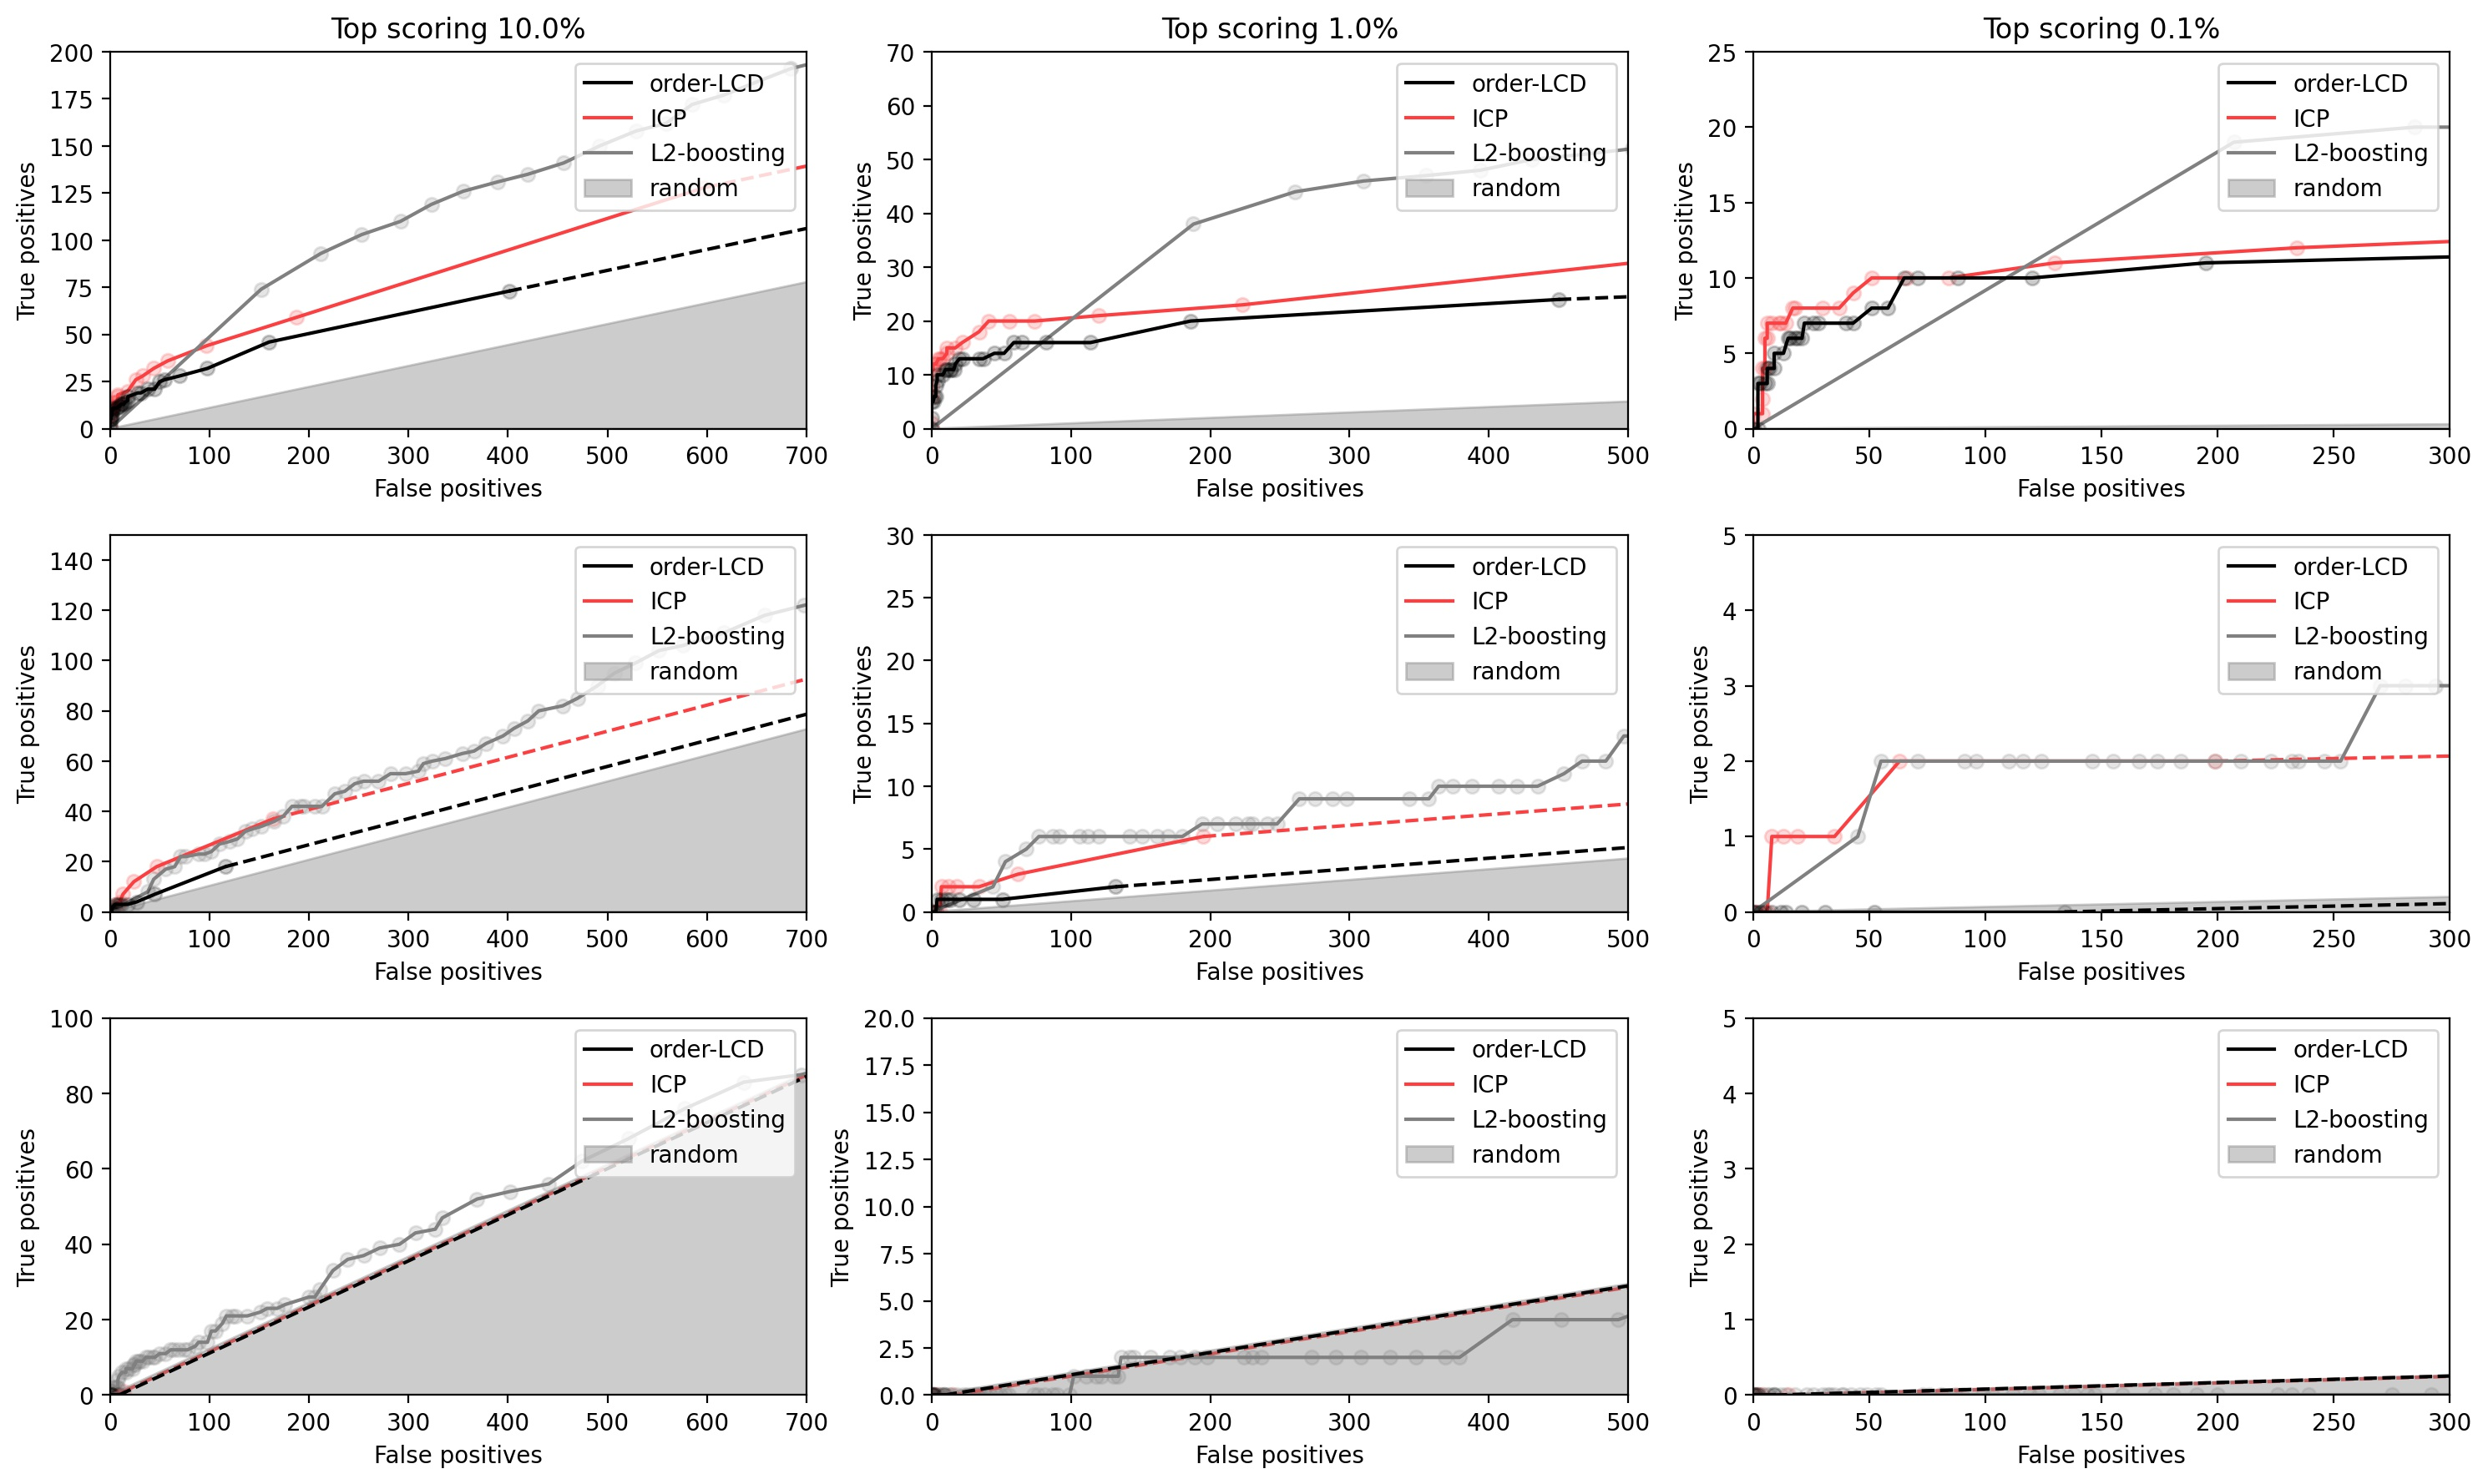
\includegraphics[width=.9\textwidth]{BROC_nor_dis_met.jpg}
    \caption{ROC curves of order-based LCD compared to other methods. \textbf{Discrete predictions} are evaluated on the \textbf{standardized ground-truth}. Columns use different ground-truth thresholds, rows different subsets of the relations that are evaluated. A dashed line indicates that a method resorts to random guessing.}
    \label{fig:app:rocversteeg}
\end{figure}
% short, norm, score
\begin{figure}[H]
    \centering
    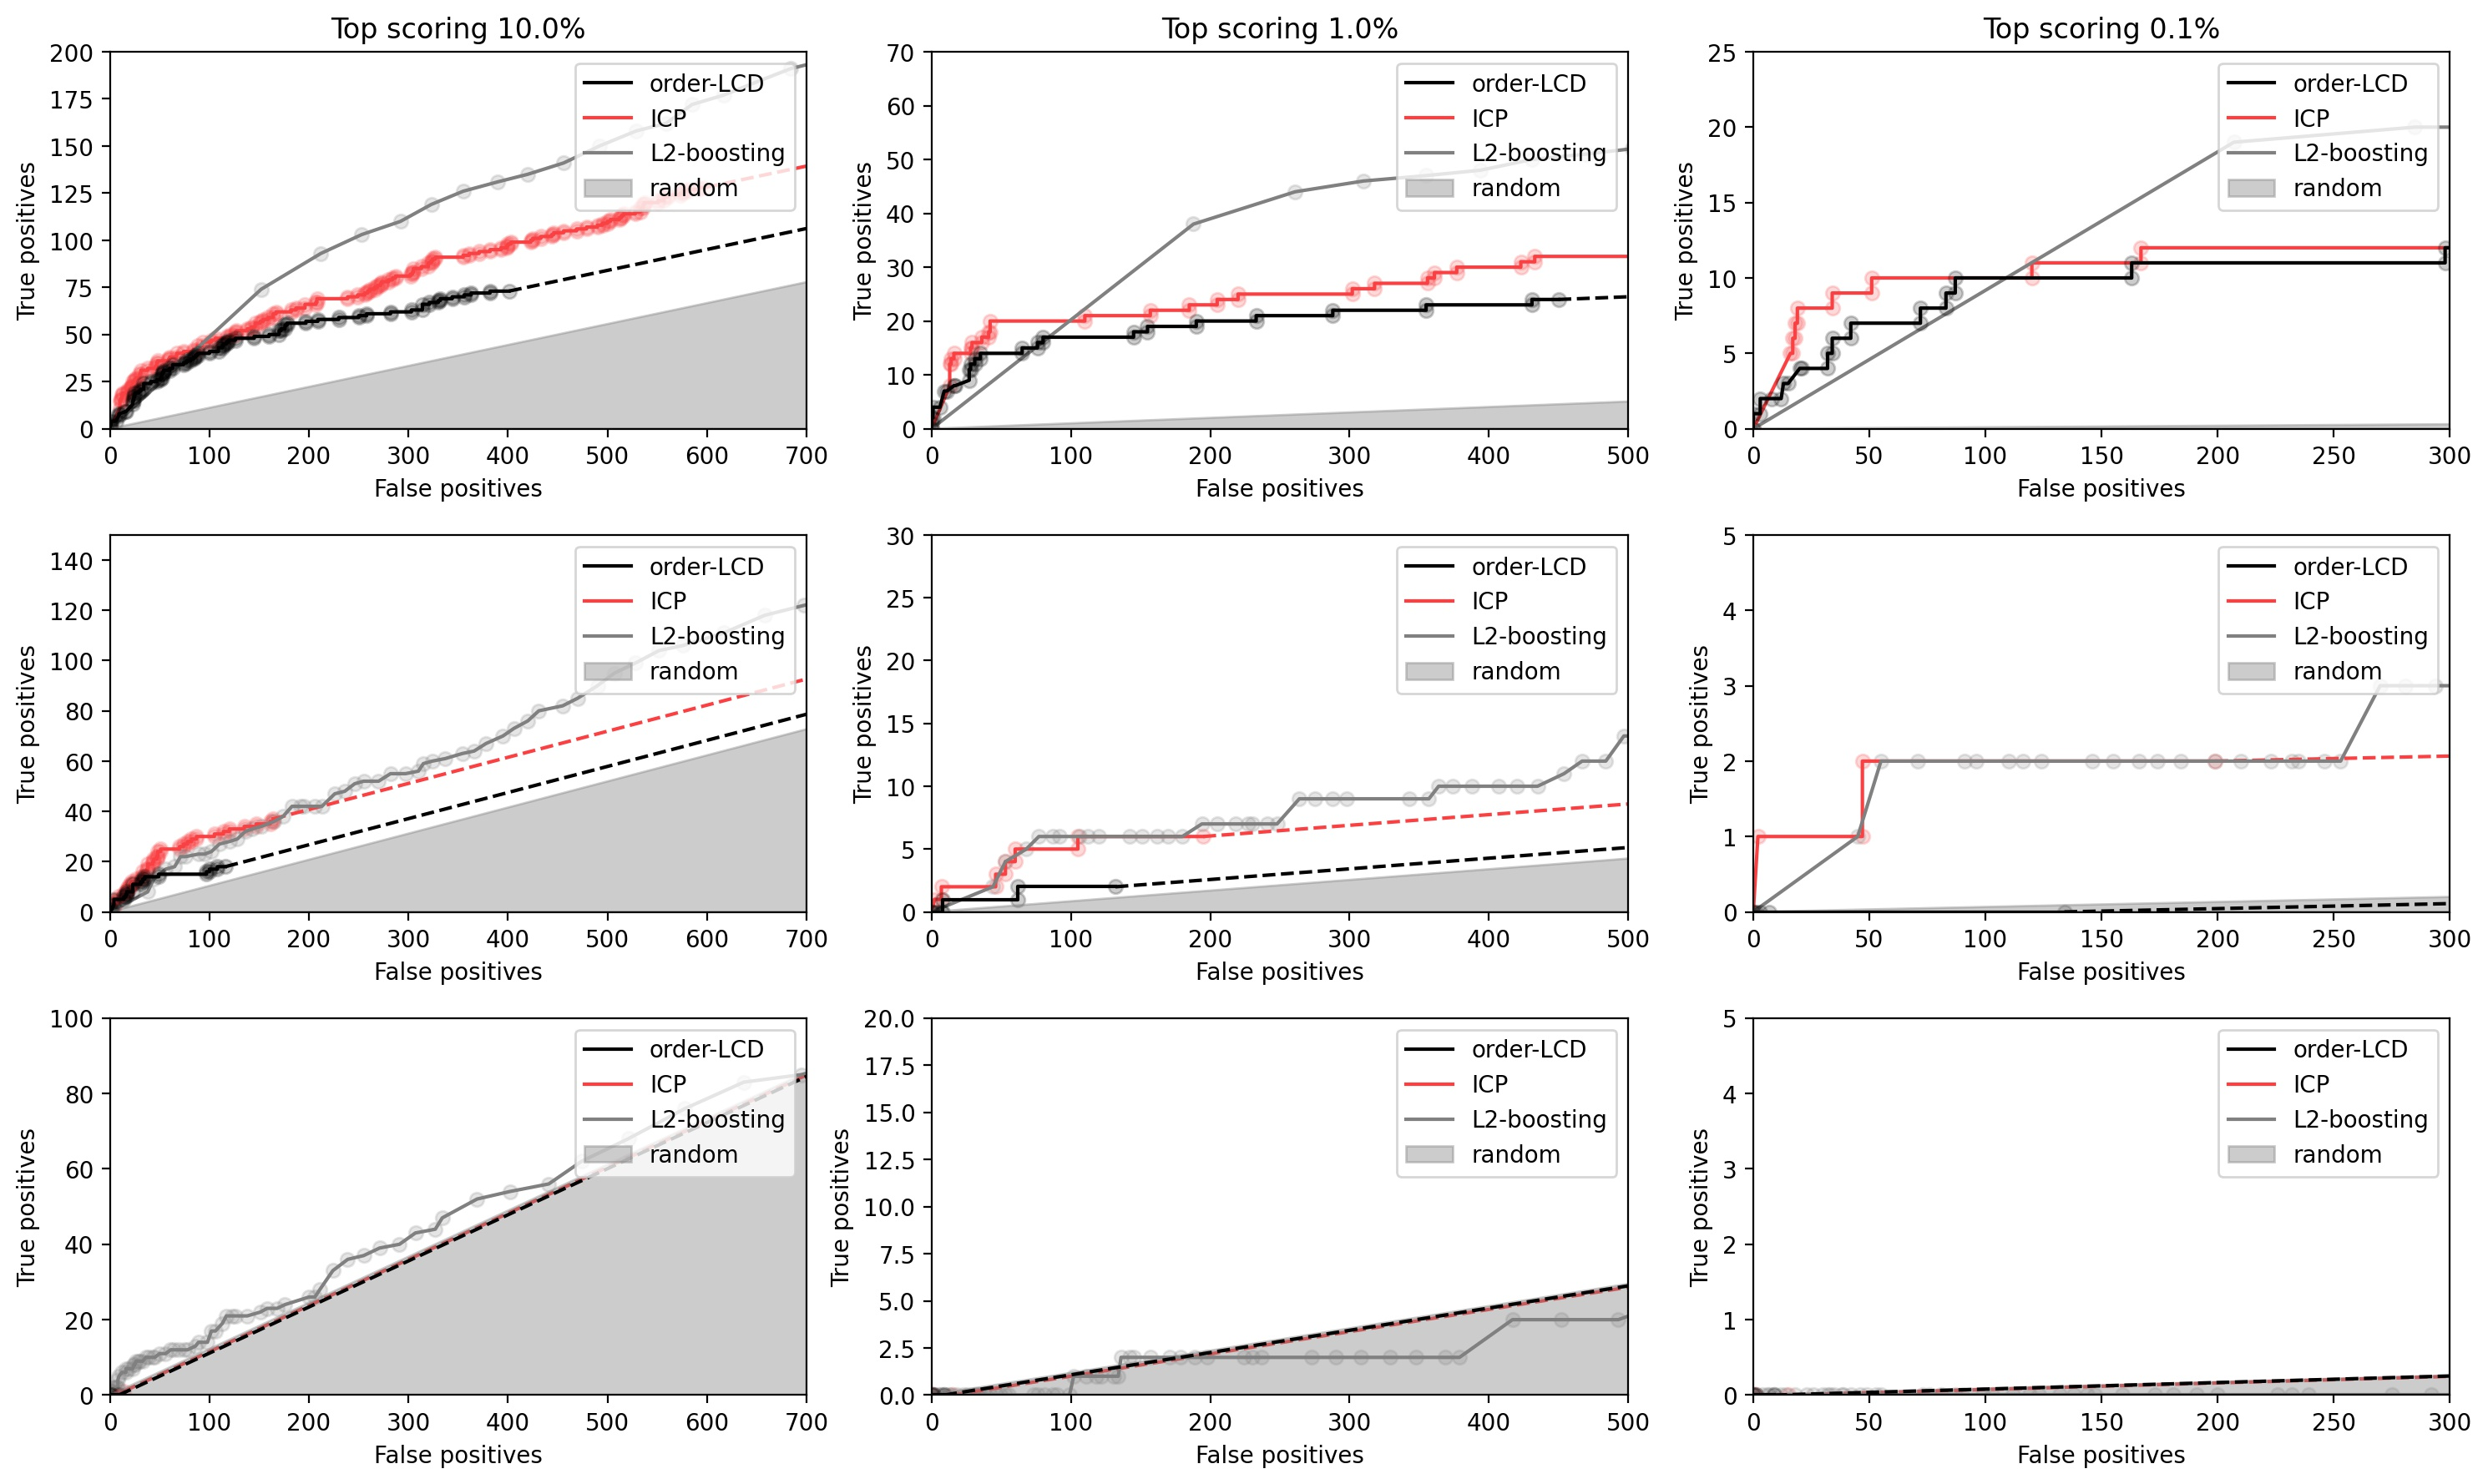
\includegraphics[width=.9\textwidth]{BROC_nor_con_met.jpg}
    \caption{ROC curves of order-based LCD compared to other methods. \textbf{Continuous predictions} are evaluated on the \textbf{standardized ground-truth}. Columns use different ground-truth thresholds, rows different subsets of the relations that are evaluated. A dashed line indicates that a method resorts to random guessing.}
\end{figure}

\subsubsection{ROC Curves Compared to LCD Methods}

% short, abs, edge
\begin{figure}[H]
    \centering
    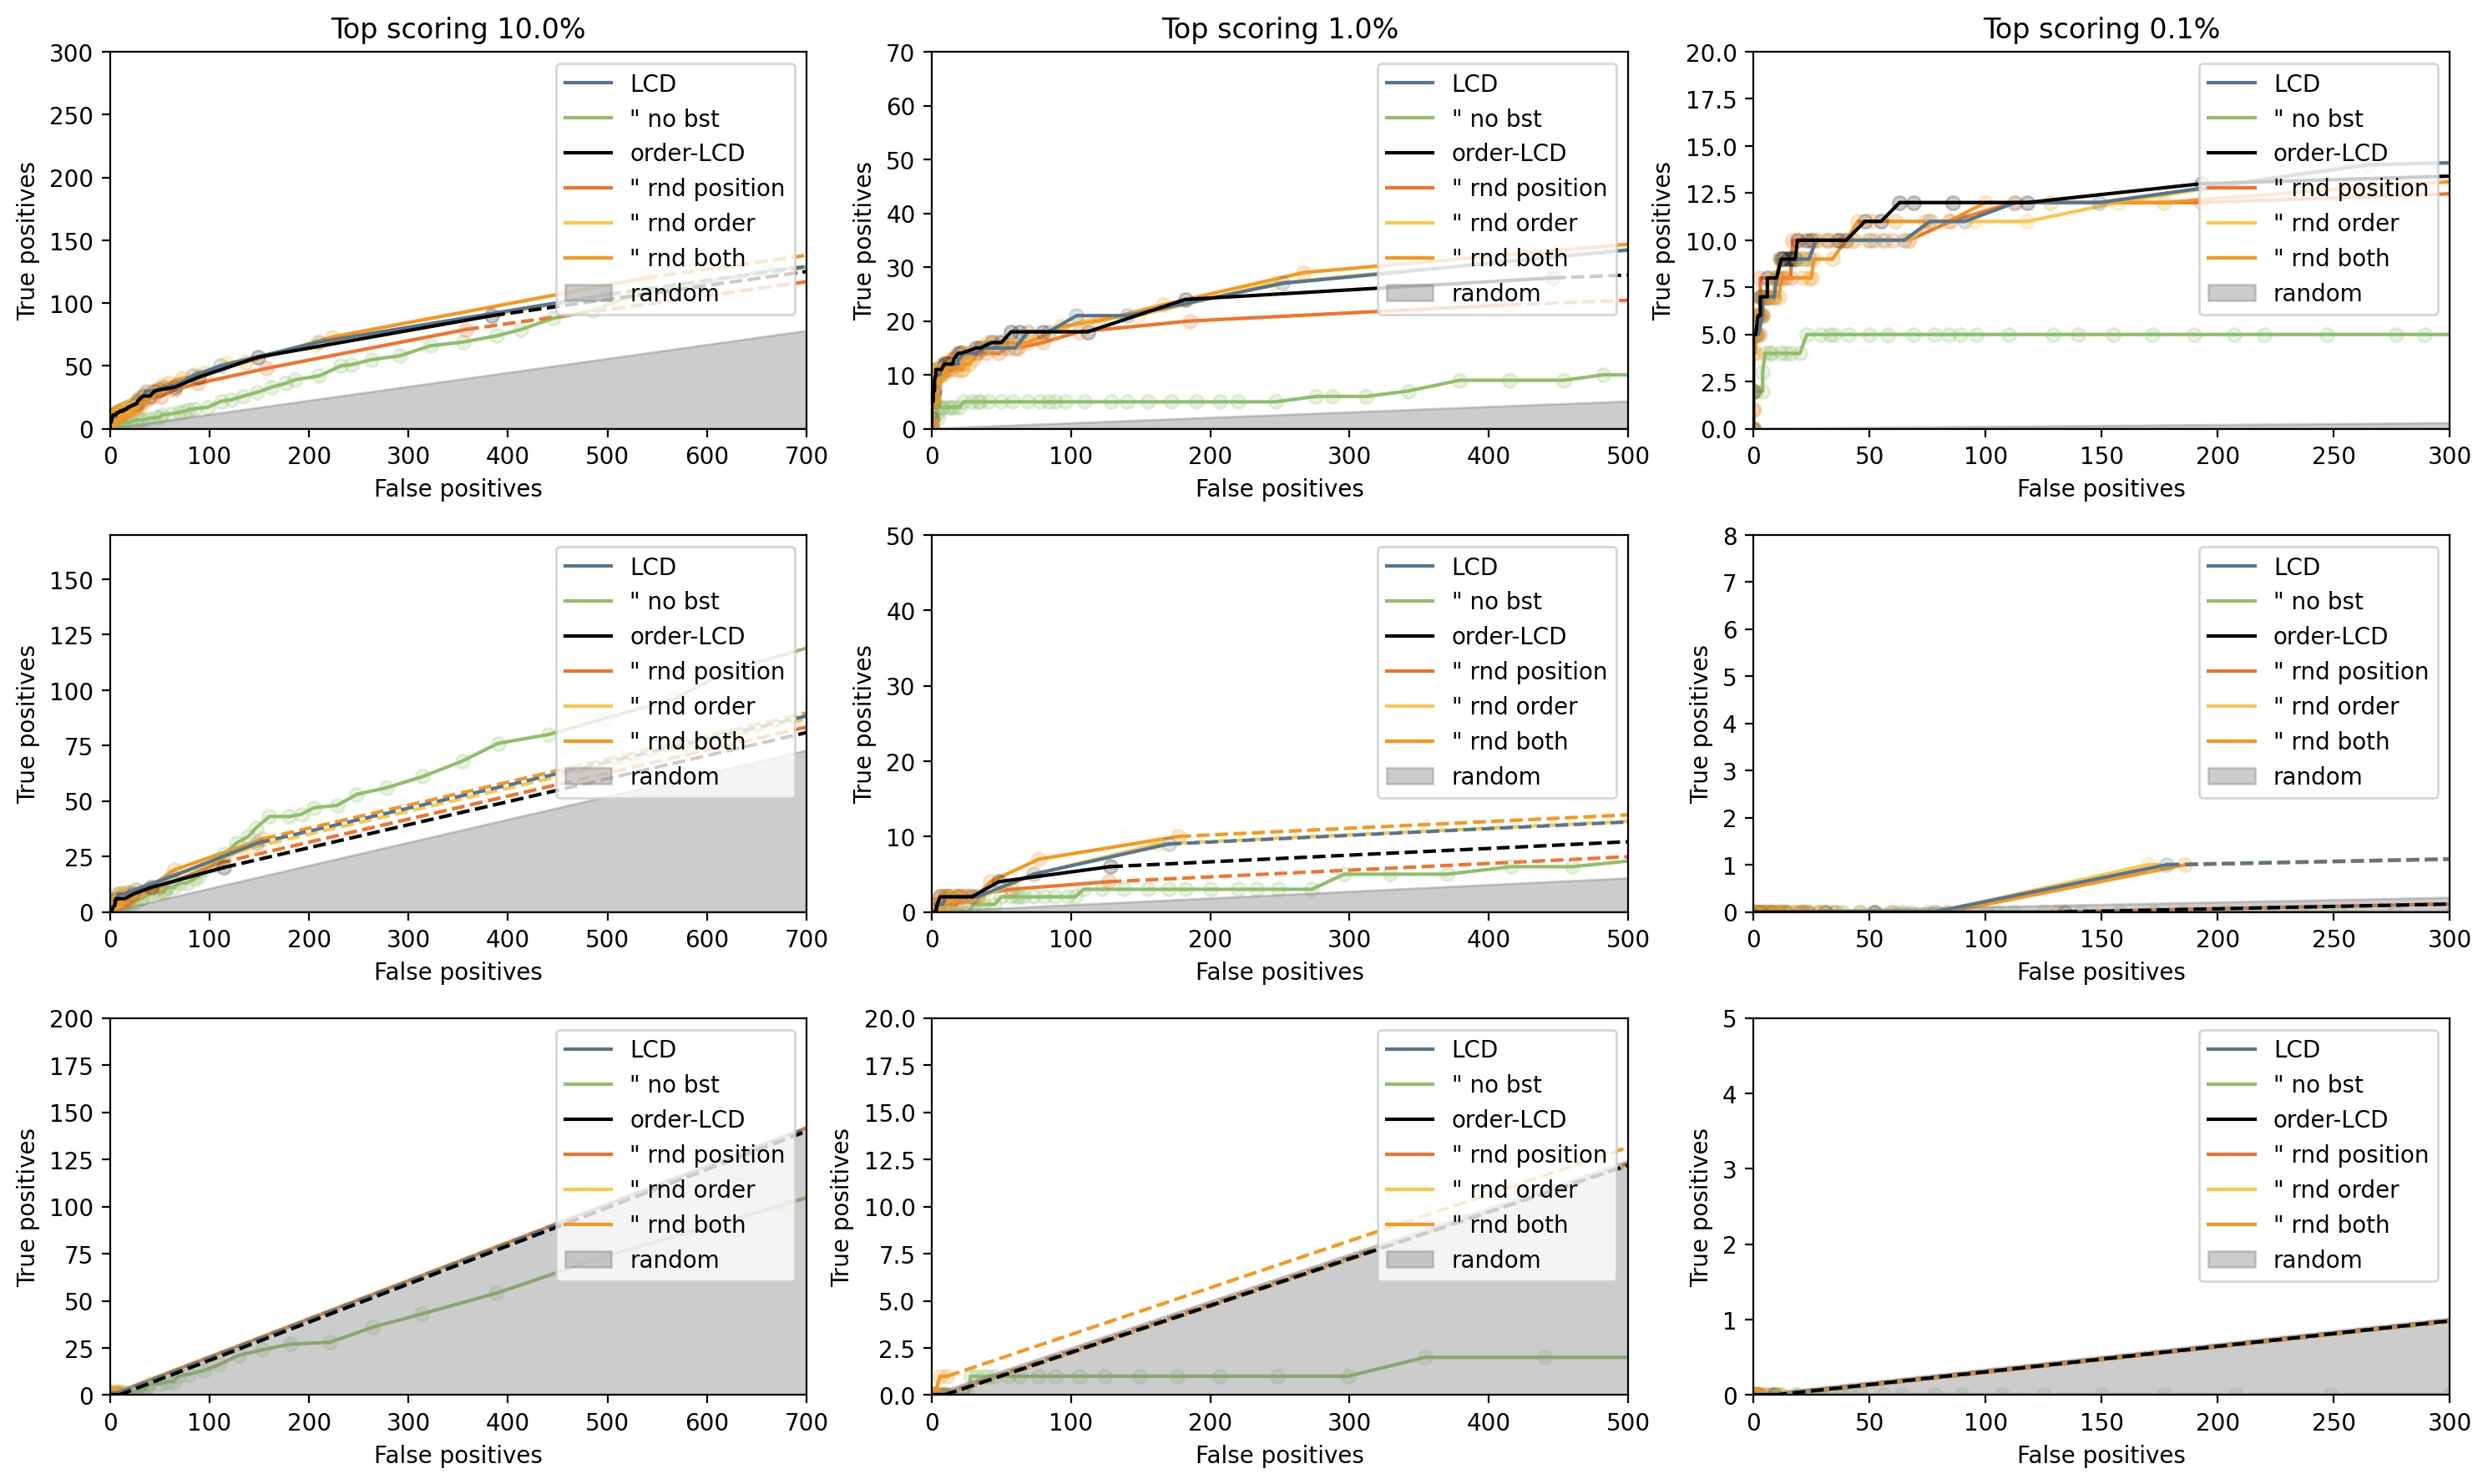
\includegraphics[width=.9\textwidth]{BROC_abs_dis_lcd.jpg}
    \caption{ROC curves of order-based LCD compared to LCD methods. \textbf{Discrete predictions} are evaluated on the \textbf{absolute ground-truth}. Columns use different ground-truth thresholds, rows different subsets of the relations that are evaluated. A dashed line indicates that a method resorts to random guessing.}
\end{figure}
% short, abs, score
\begin{figure}[H]
    \centering
    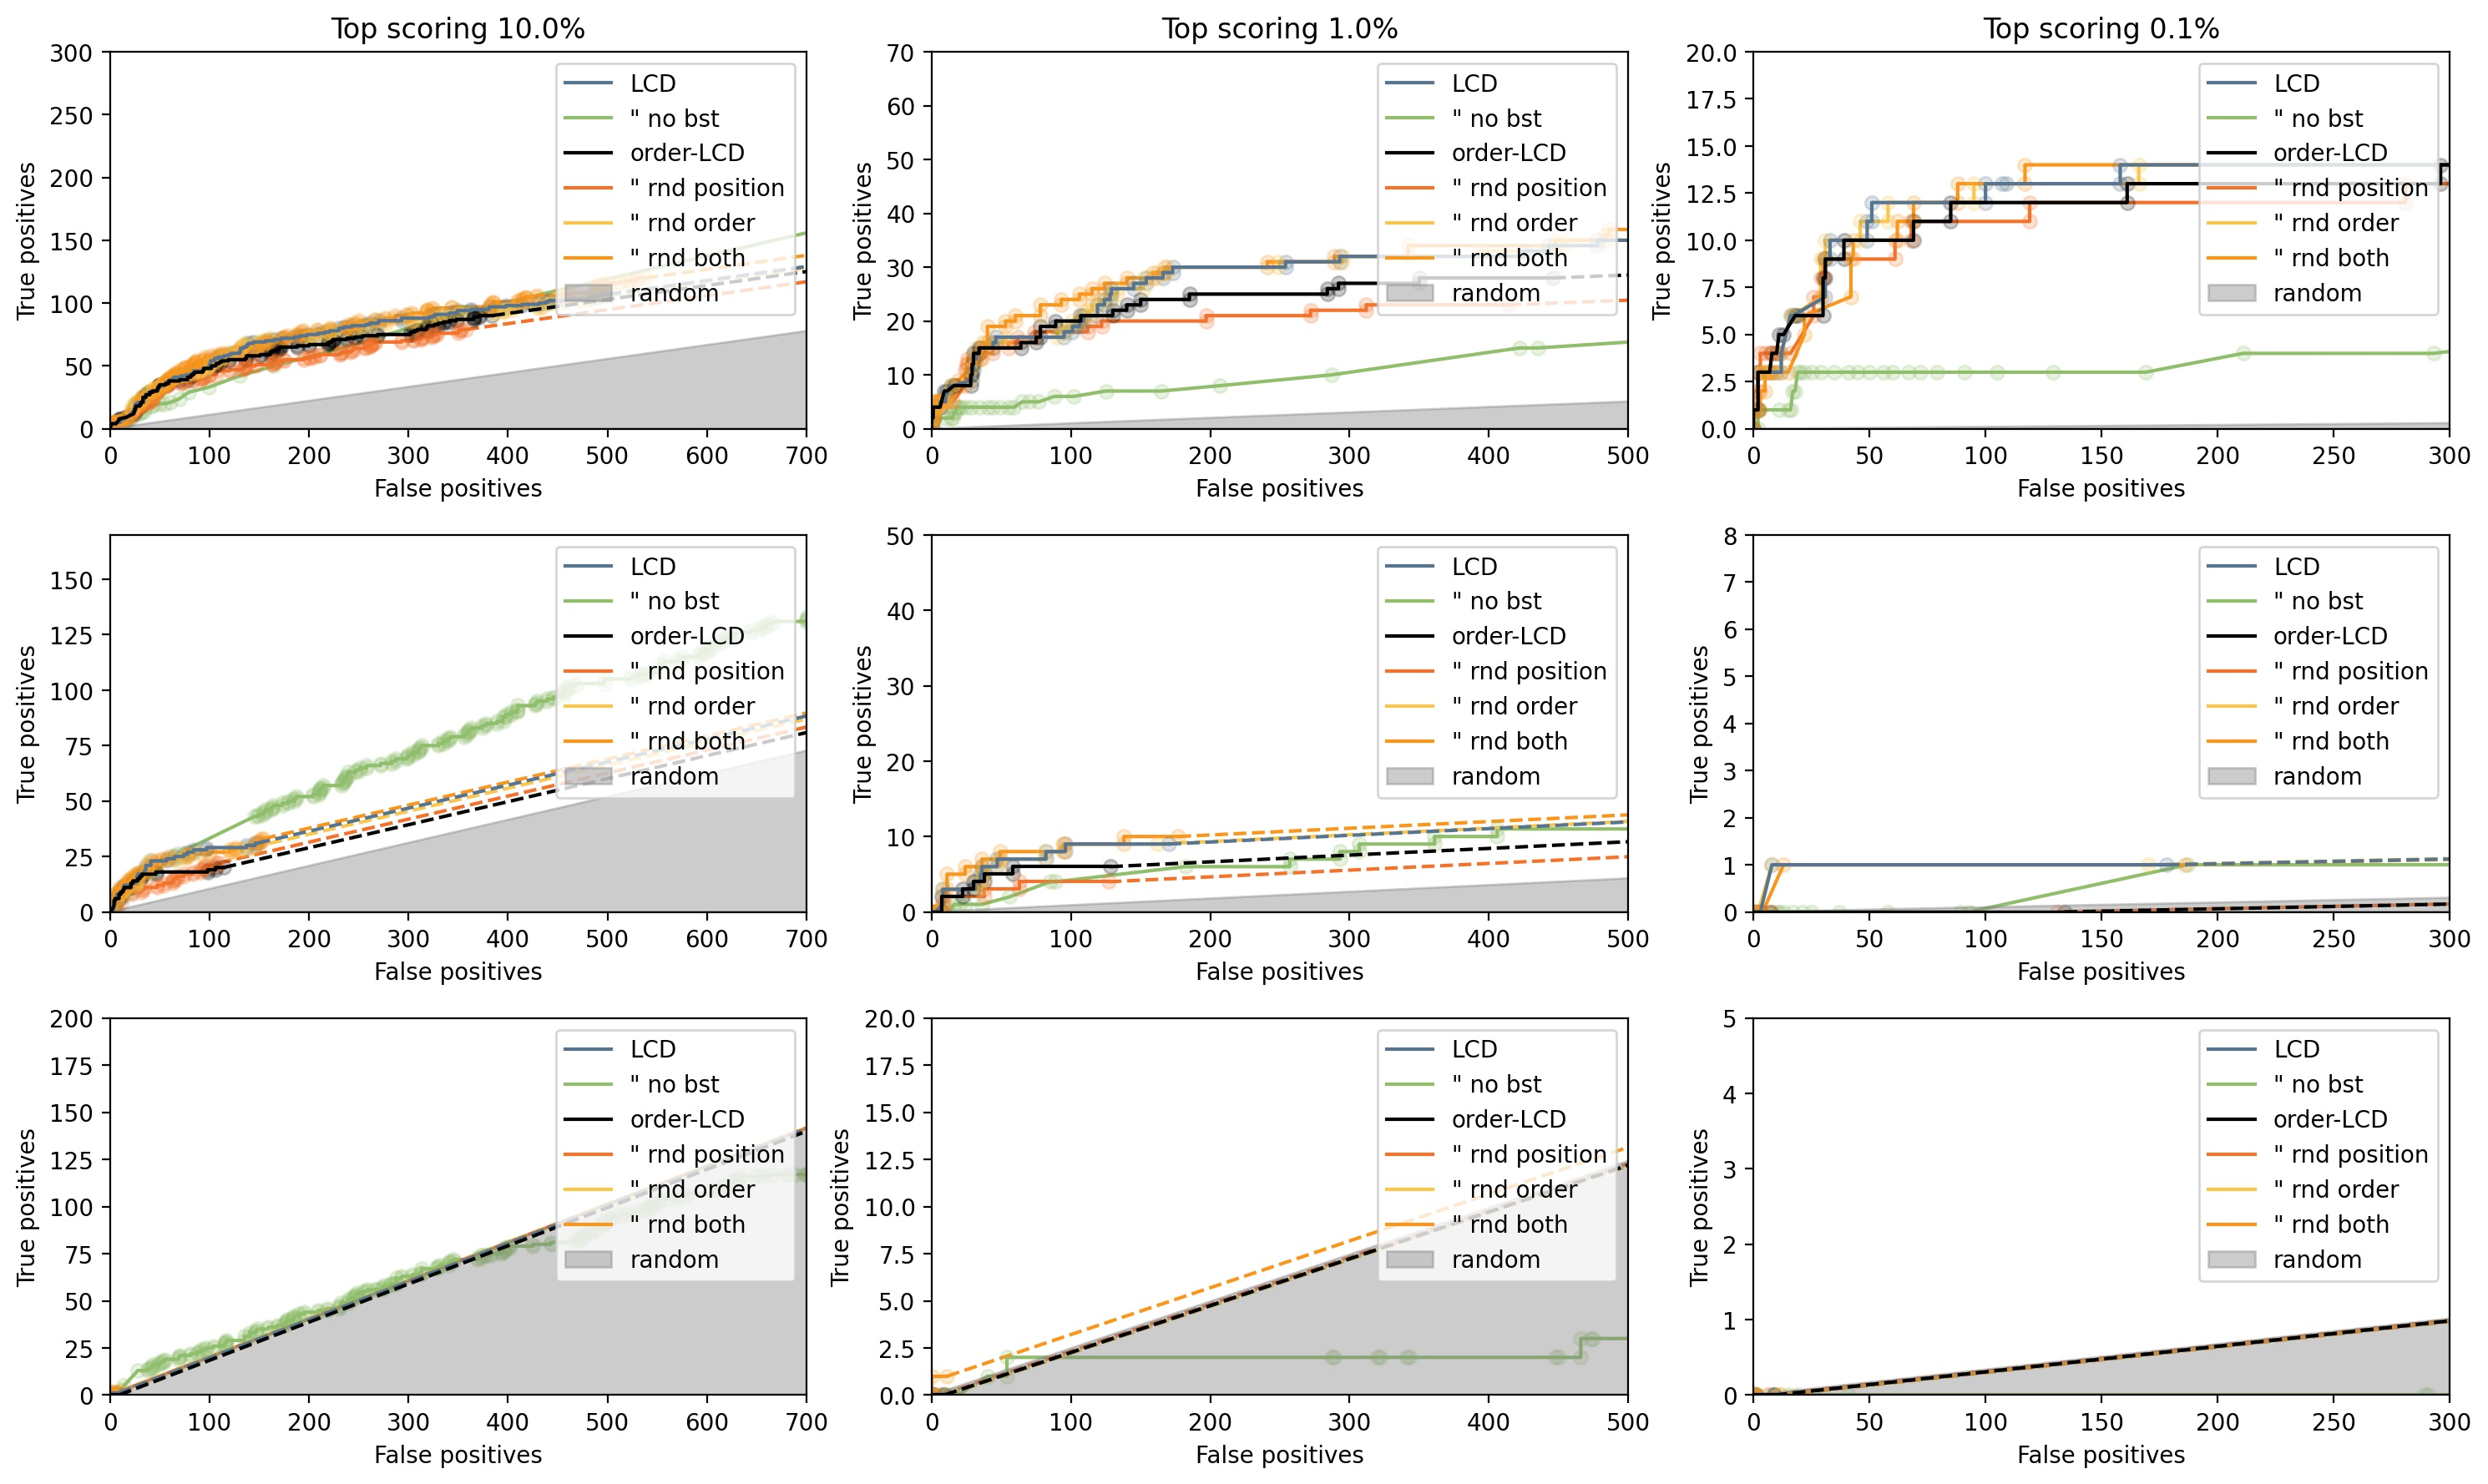
\includegraphics[width=.9\textwidth]{BROC_abs_con_lcd.jpg}
    \caption{ROC curves of order-based LCD compared to LCD methods. \textbf{Continuous predictions} are evaluated on the \textbf{absolute ground-truth}. Columns use different ground-truth thresholds, rows different subsets of the relations that are evaluated. A dashed line indicates that a method resorts to random guessing.}
\end{figure}
% short, norm, edge
\begin{figure}[H]
    \centering
    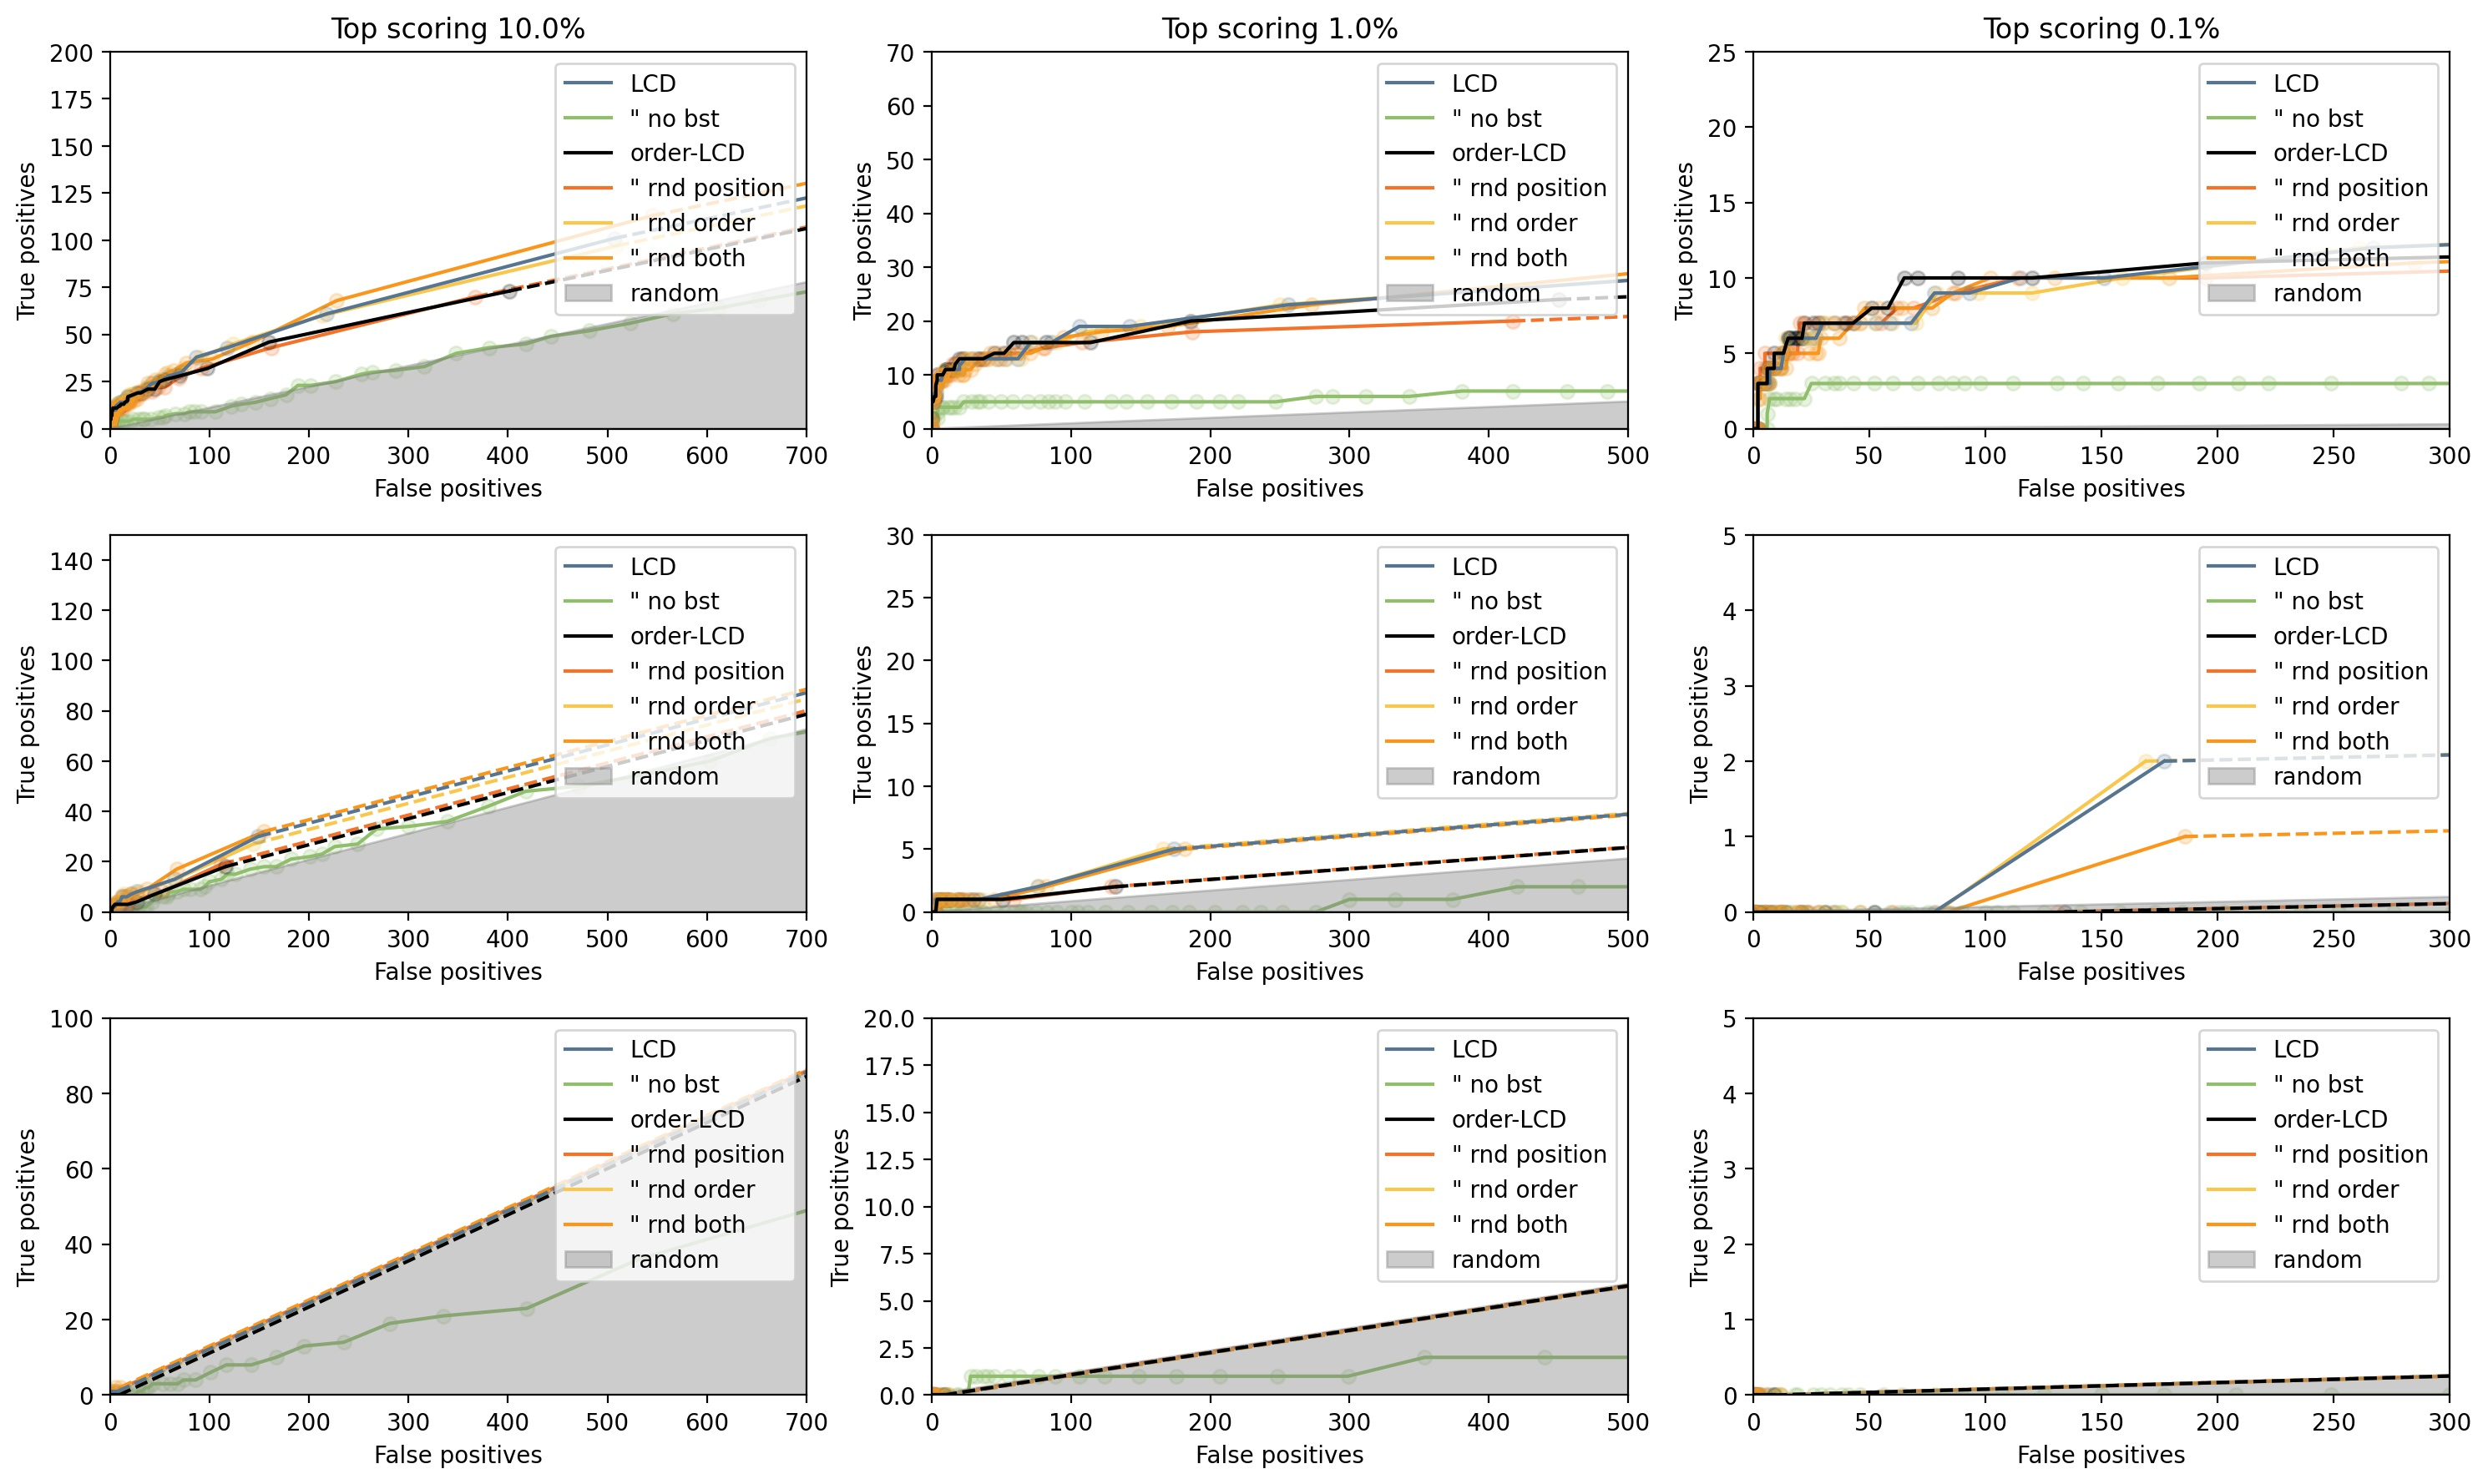
\includegraphics[width=.9\textwidth]{BROC_nor_dis_lcd.jpg}
    \caption{ROC curves of order-based LCD compared to LCD methods. \textbf{Discrete predictions} are evaluated on the \textbf{standardized ground-truth}. Columns use different ground-truth thresholds, rows different subsets of the relations that are evaluated. A dashed line indicates that a method resorts to random guessing.}
\end{figure}
% short, norm, score
\begin{figure}[H]
    \centering
    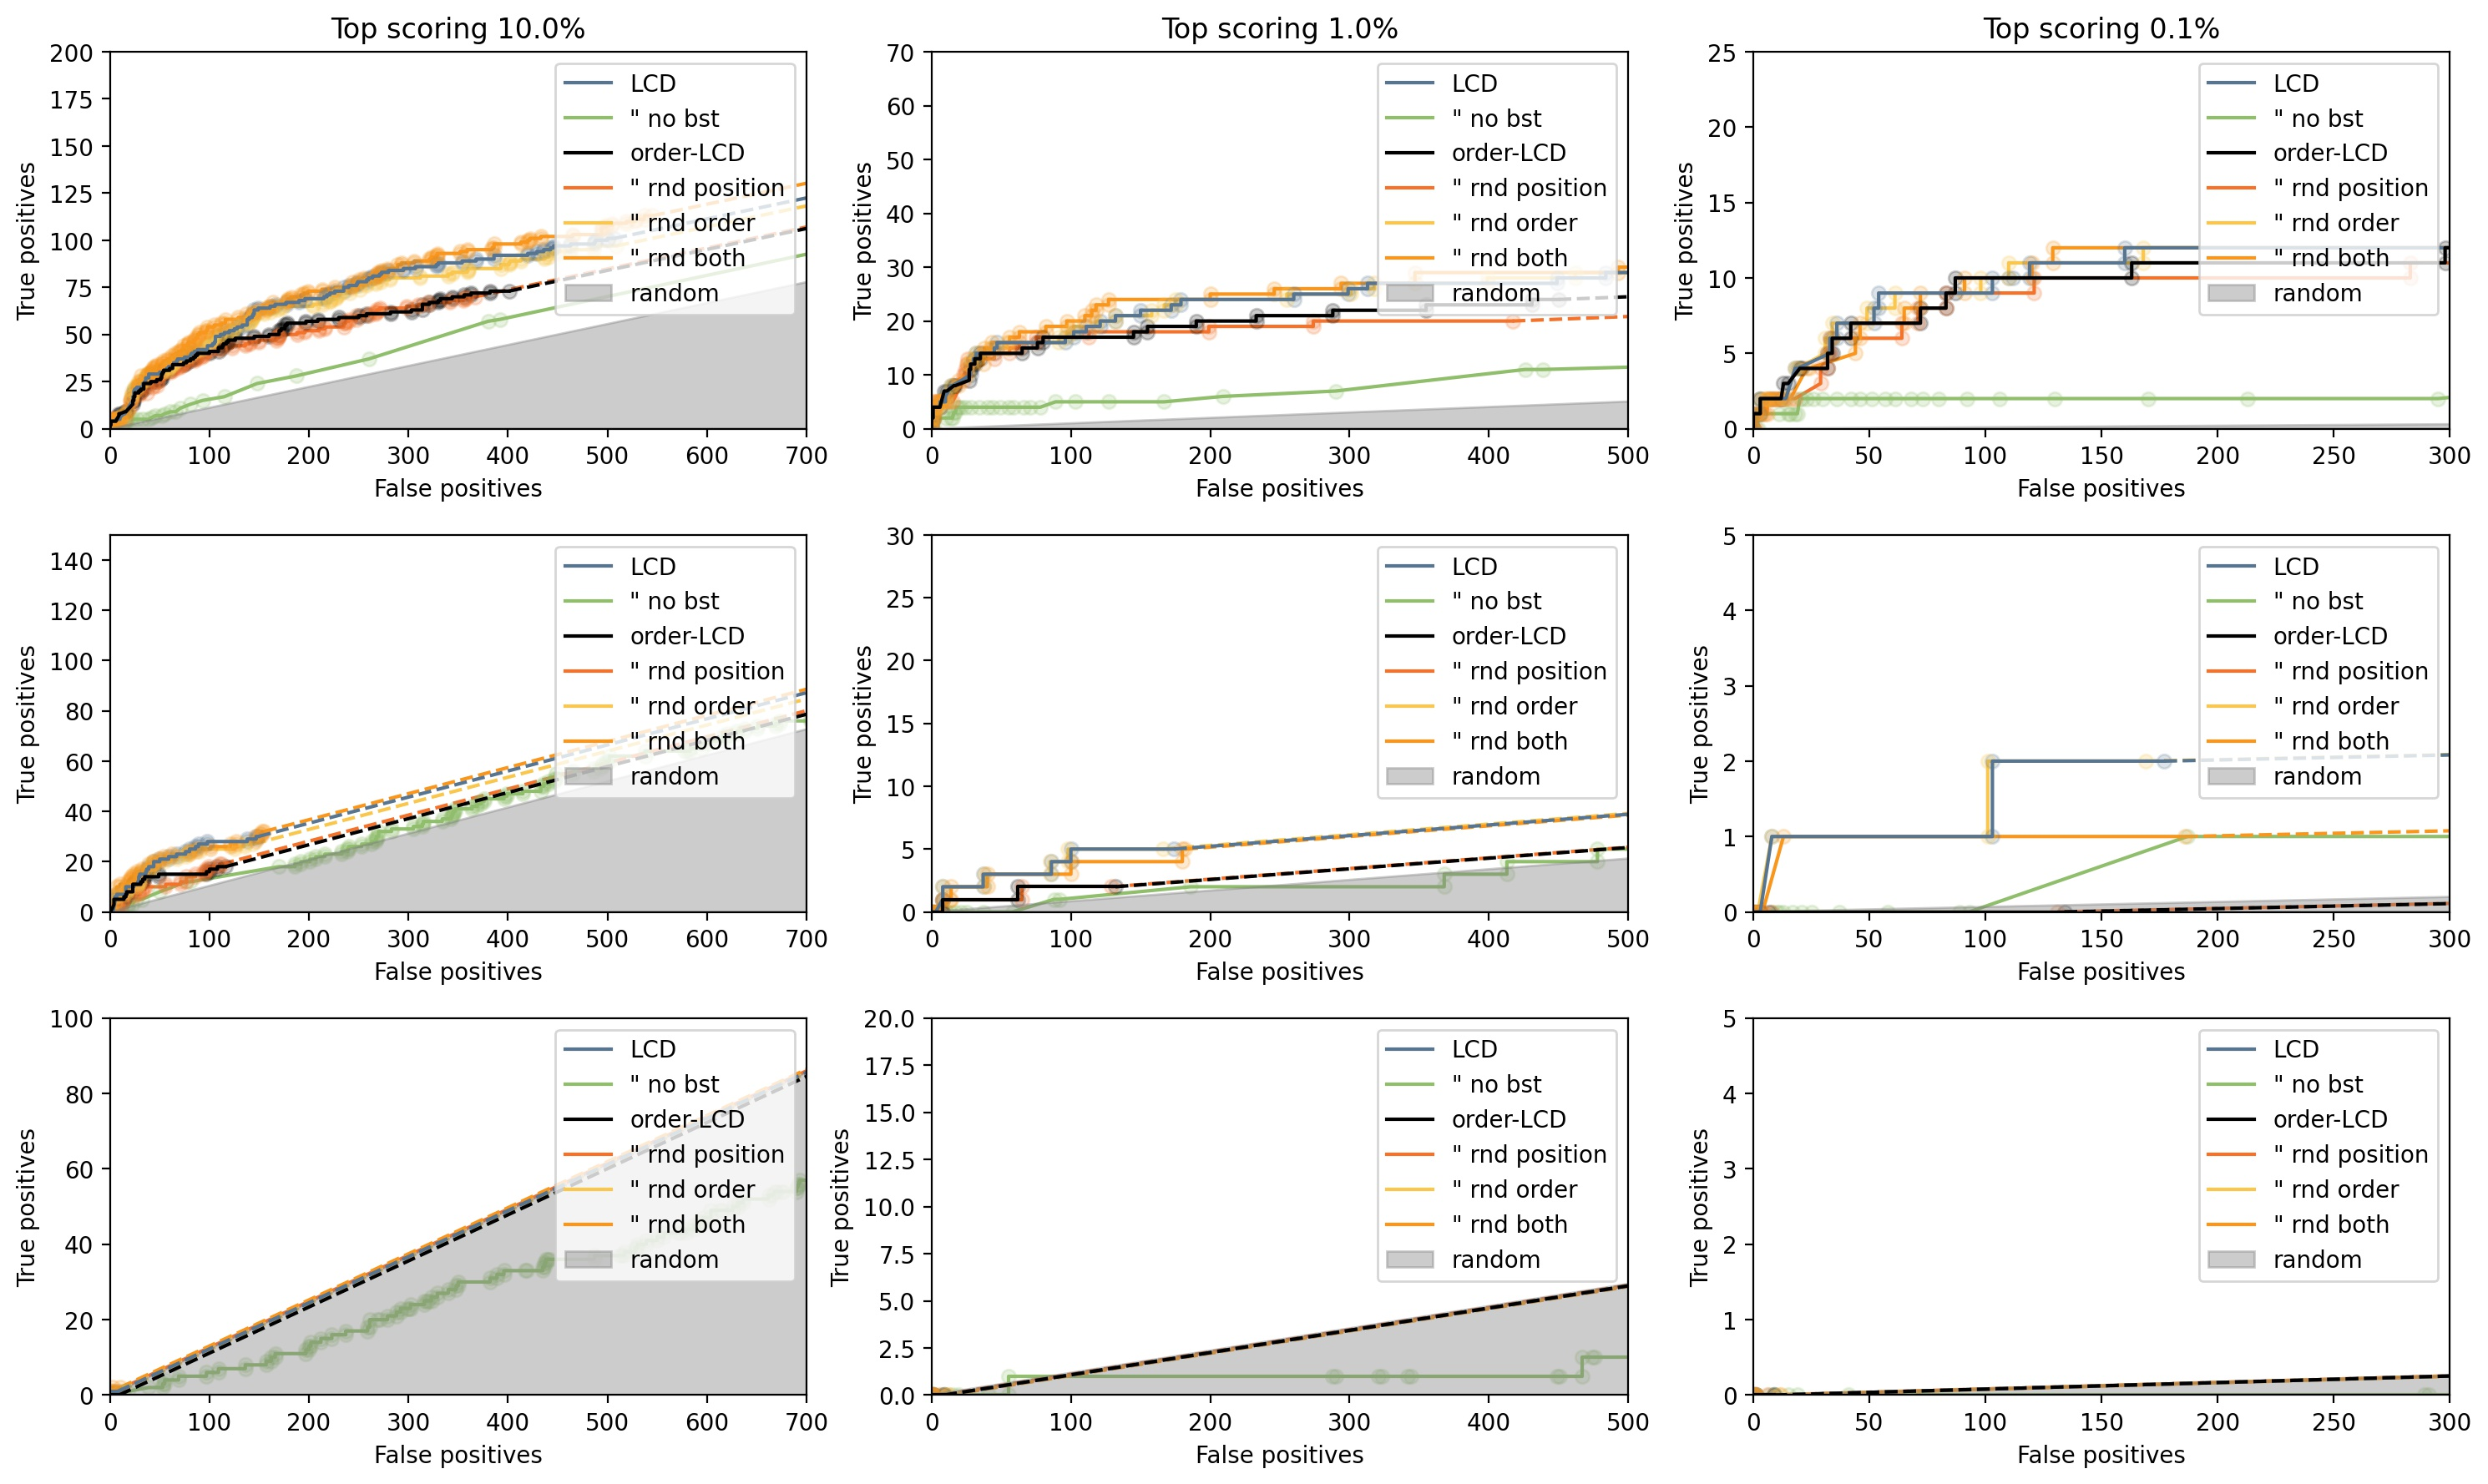
\includegraphics[width=.9\textwidth]{BROC_nor_con_lcd.jpg}
    \caption{ROC curves of order-based LCD compared to LCD methods. \textbf{Continuous predictions} are evaluated on the \textbf{standardized ground-truth}. Columns use different ground-truth thresholds, rows different subsets of the relations that are evaluated. A dashed line indicates that a method resorts to random guessing.}
\end{figure}


\subsubsection{Inclusive and Exclusive Order-Based LCD and LCD Relations}

% order, inclusive
\begin{figure}[H]
    \centering
    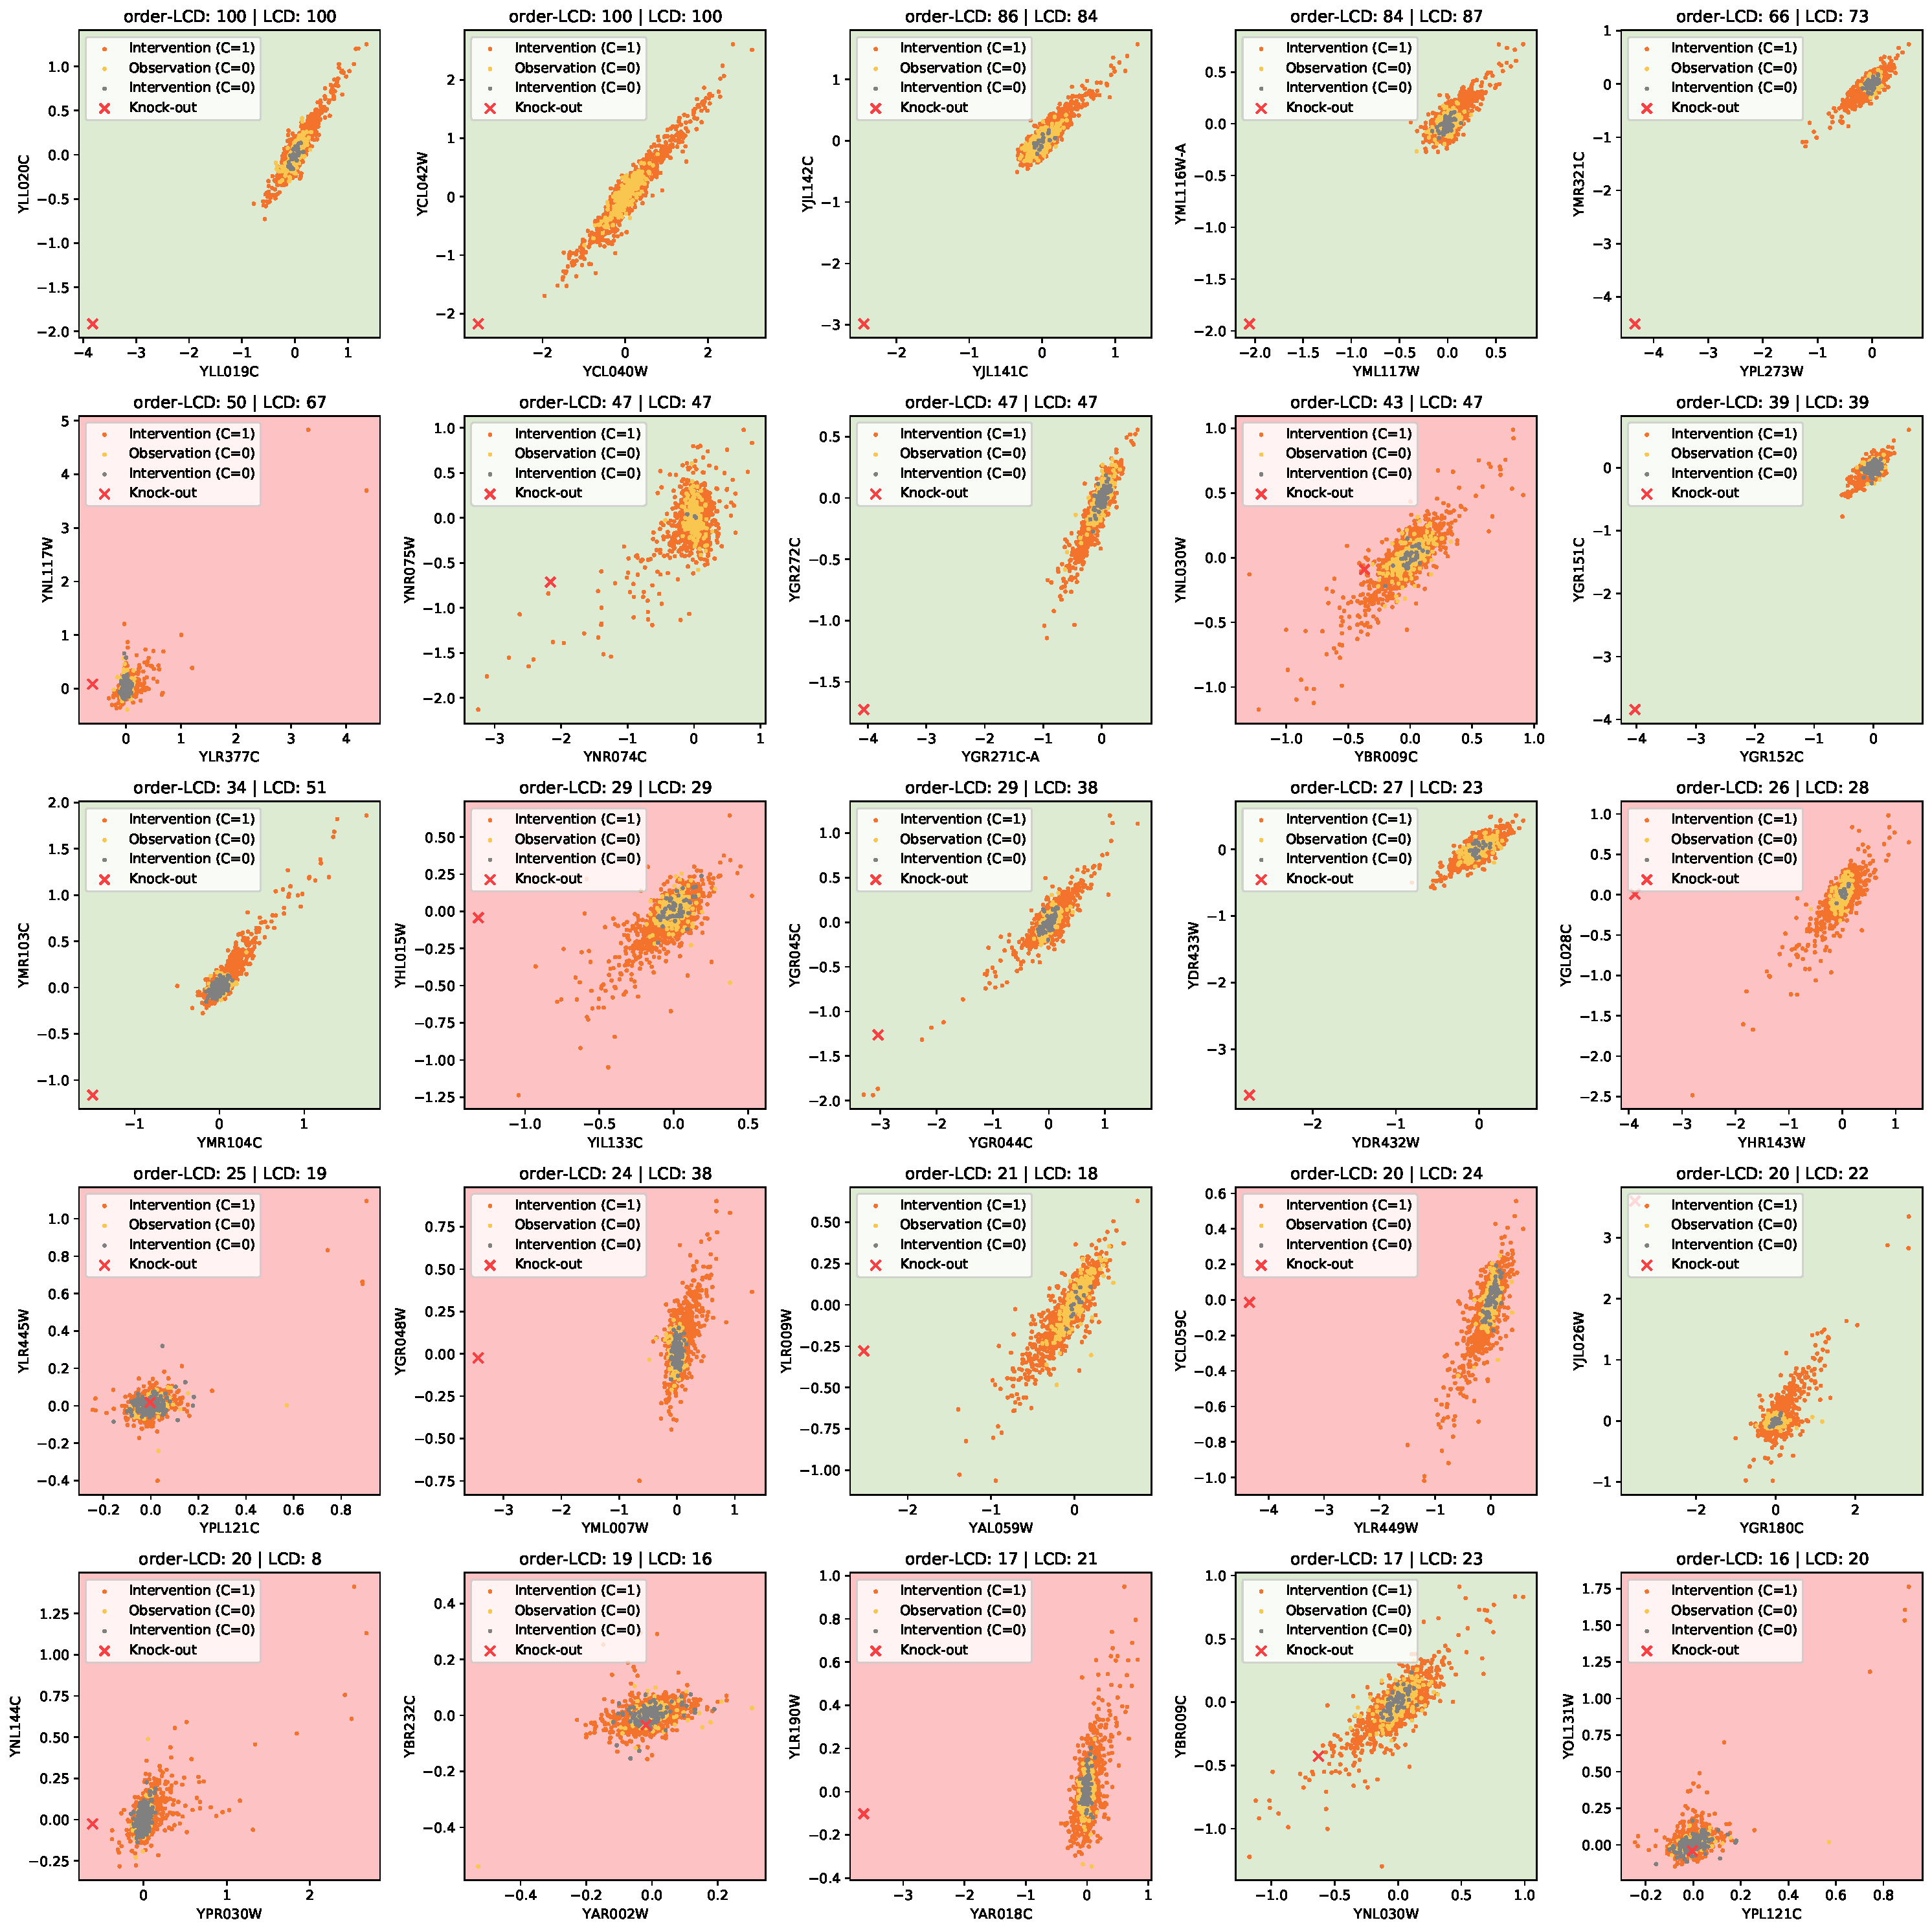
\includegraphics[width=\textwidth]{Binclusive_olcd.pdf}
    \caption{The 25 strongest predictions by \textbf{order-based LCD} that are also \textbf{included} in the LCD predictions. The precise scores are shown above the figures. The background color indicates whether the relation is true according to the $10\%$ threshold.}
\end{figure}

% lcd, inclusive
\begin{figure}[H]
    \centering
    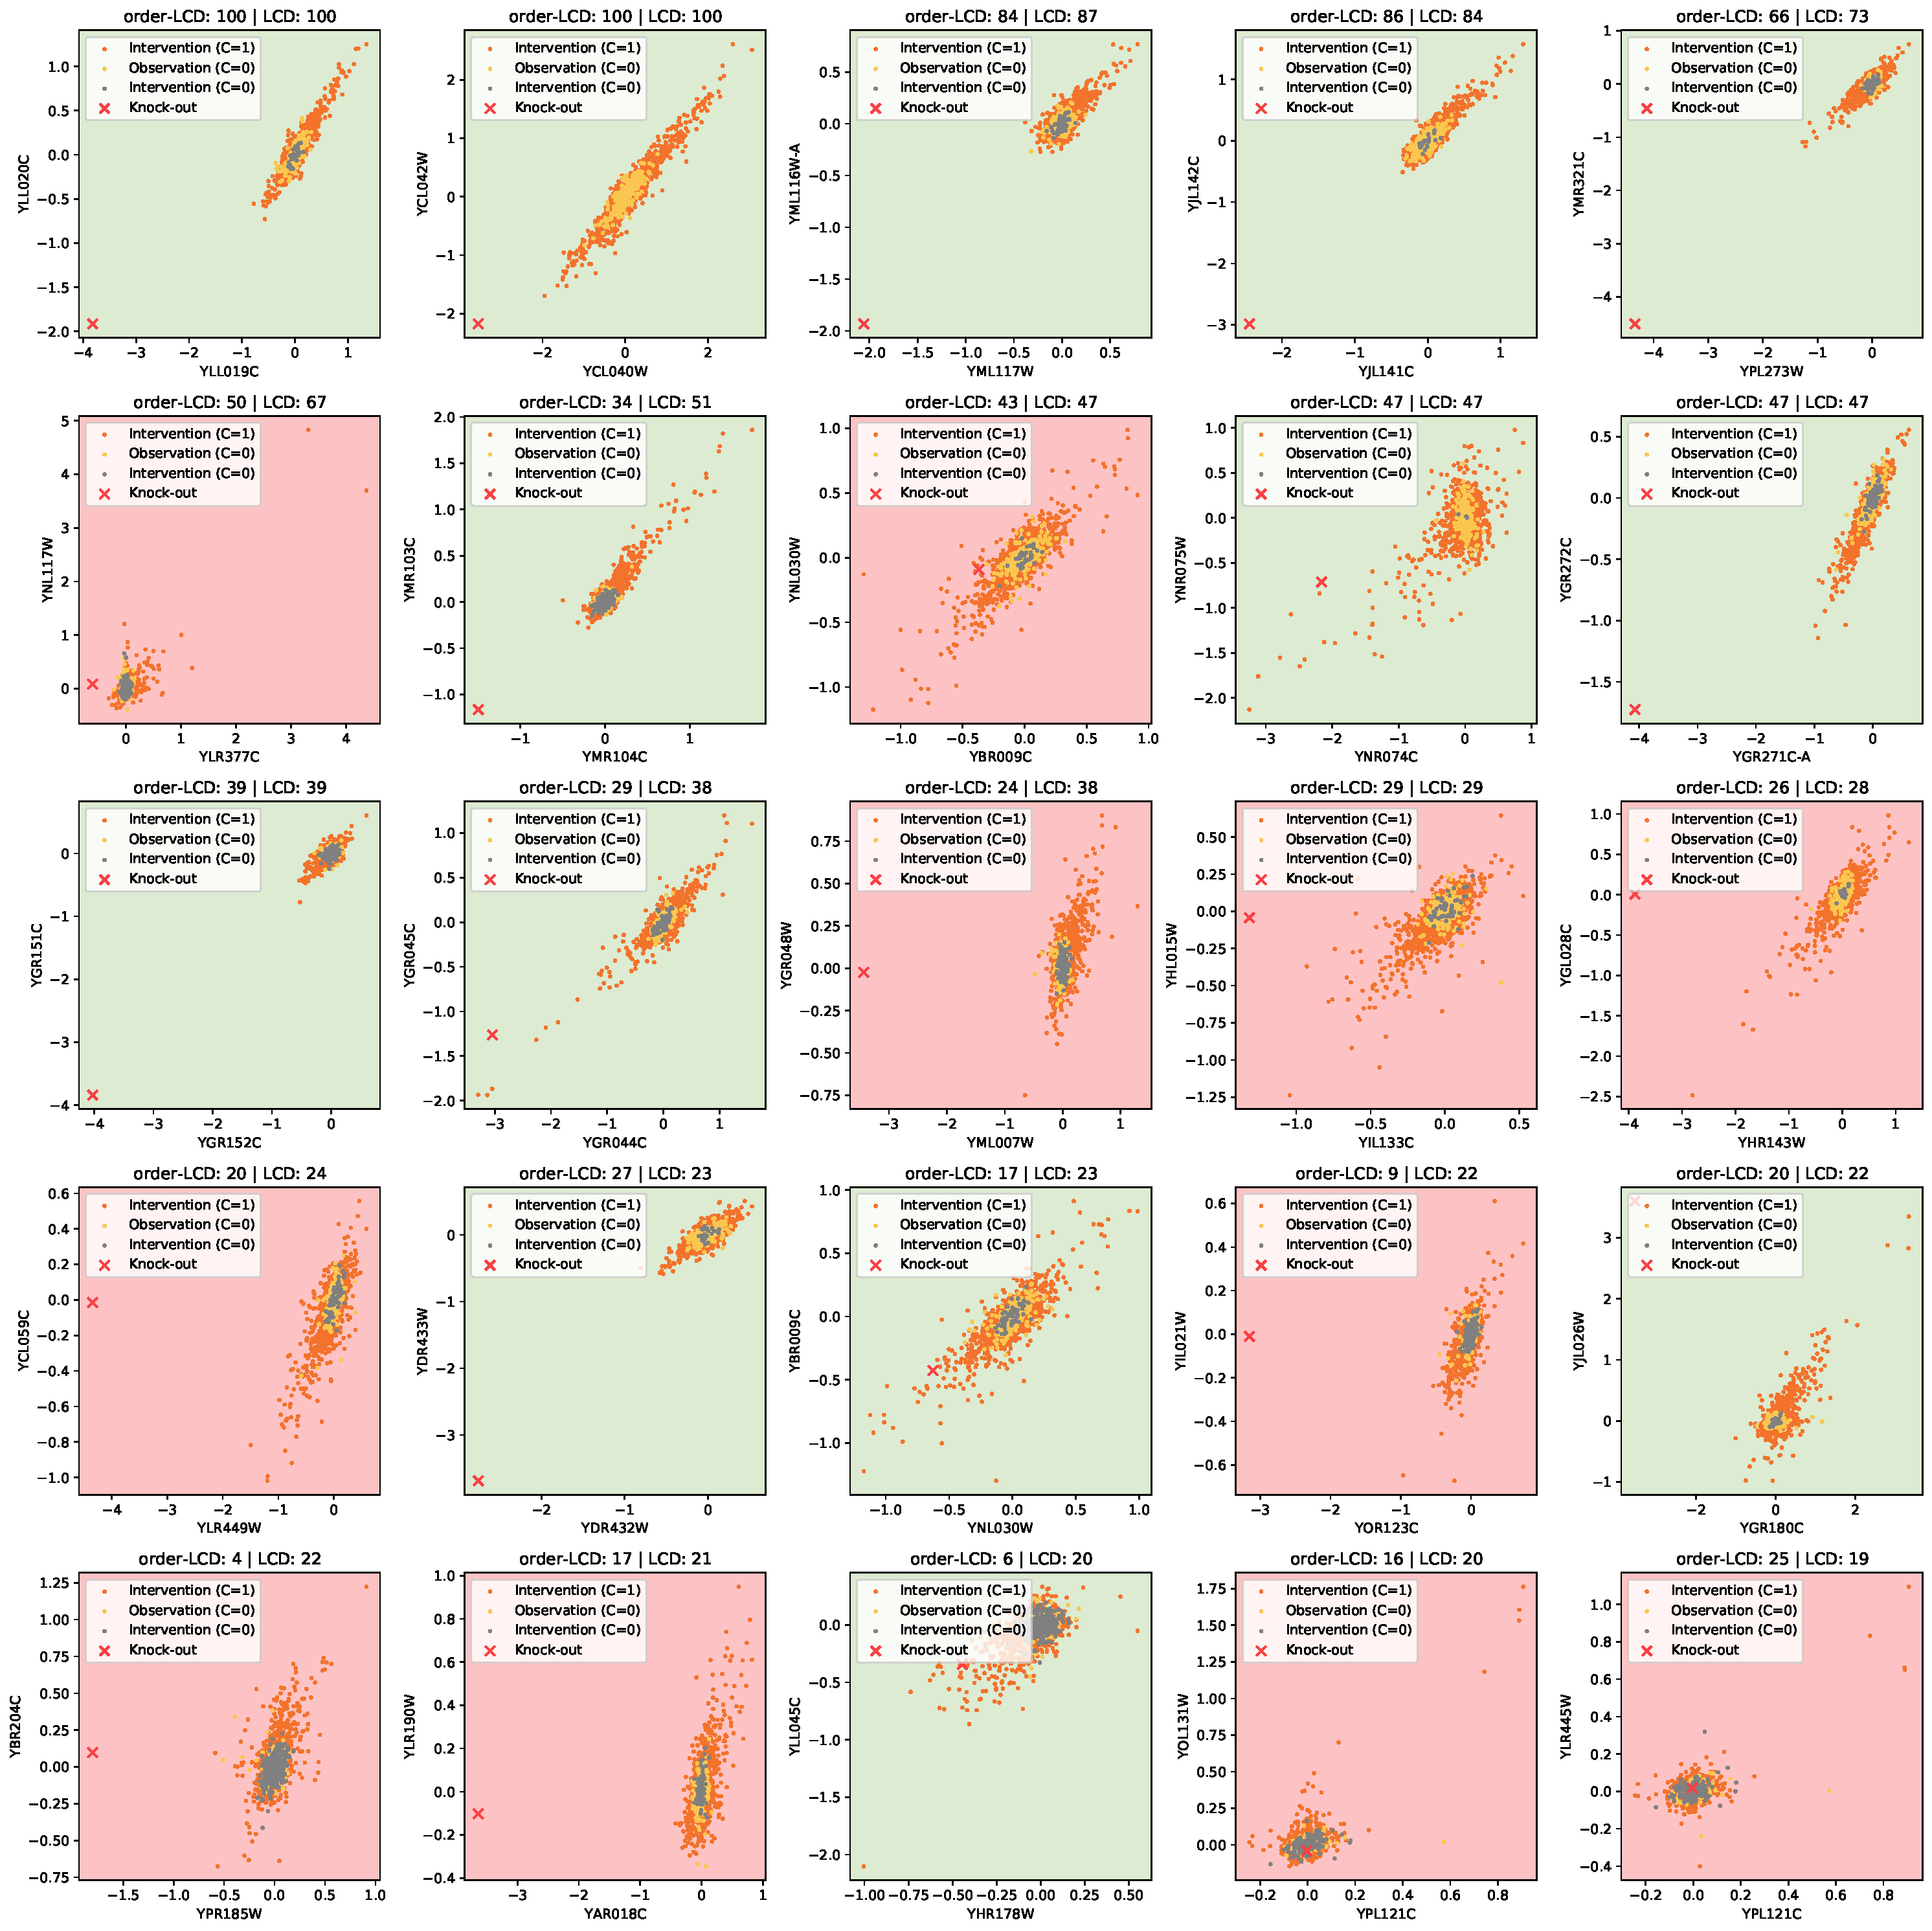
\includegraphics[width=\textwidth]{Binclusive_lcd.pdf}
    \caption{The 25 strongest predictions by \textbf{LCD} that are also \textbf{included} in the order-based LCD predictions. The precise scores are shown above the figures. The background color indicates whether the relation is true according to the $10\%$ threshold.}
\end{figure}

% order, inclusive
\begin{figure}[H]
    \centering
    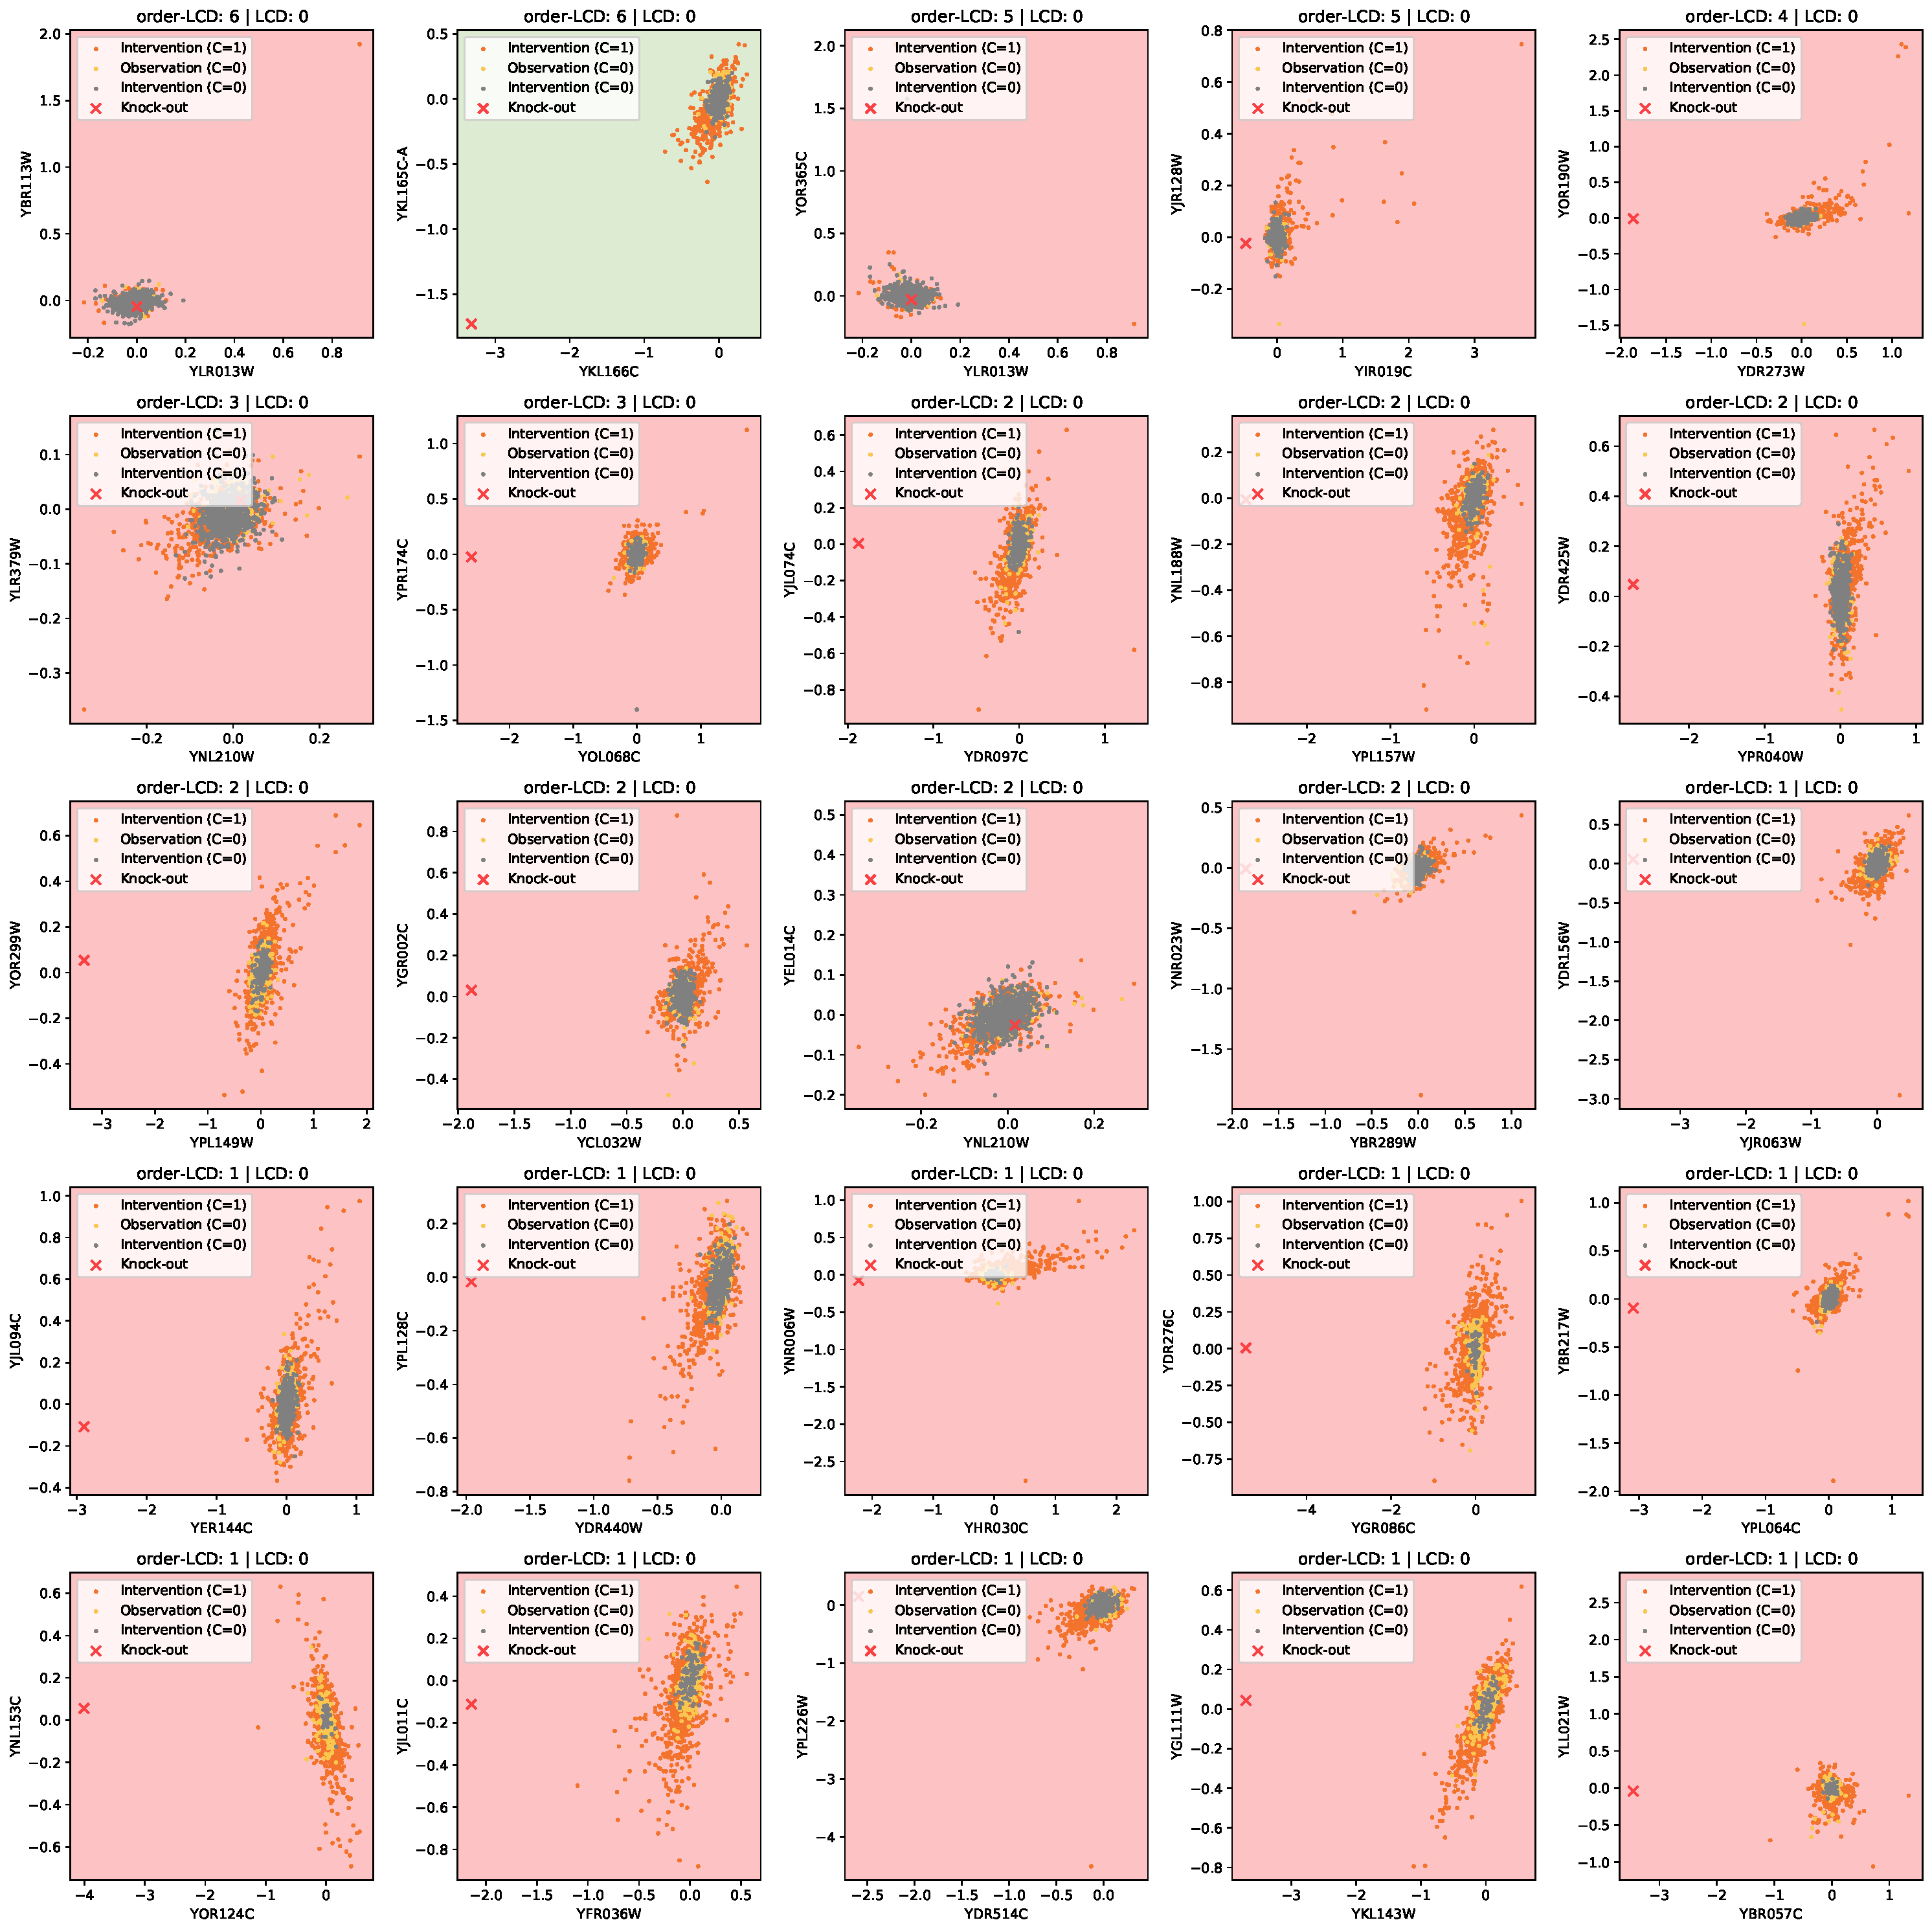
\includegraphics[width=\textwidth]{Bexclusive_olcd.pdf}
    \caption{The 25 strongest predictions by \textbf{order-based LCD} that are \textbf{excluded} in the LCD predictions. The precise scores are shown above the figures. The background color indicates whether the relation is true according to the $10\%$ threshold.}
\end{figure}

% lcd, inclusive
\begin{figure}[H]
    \centering
    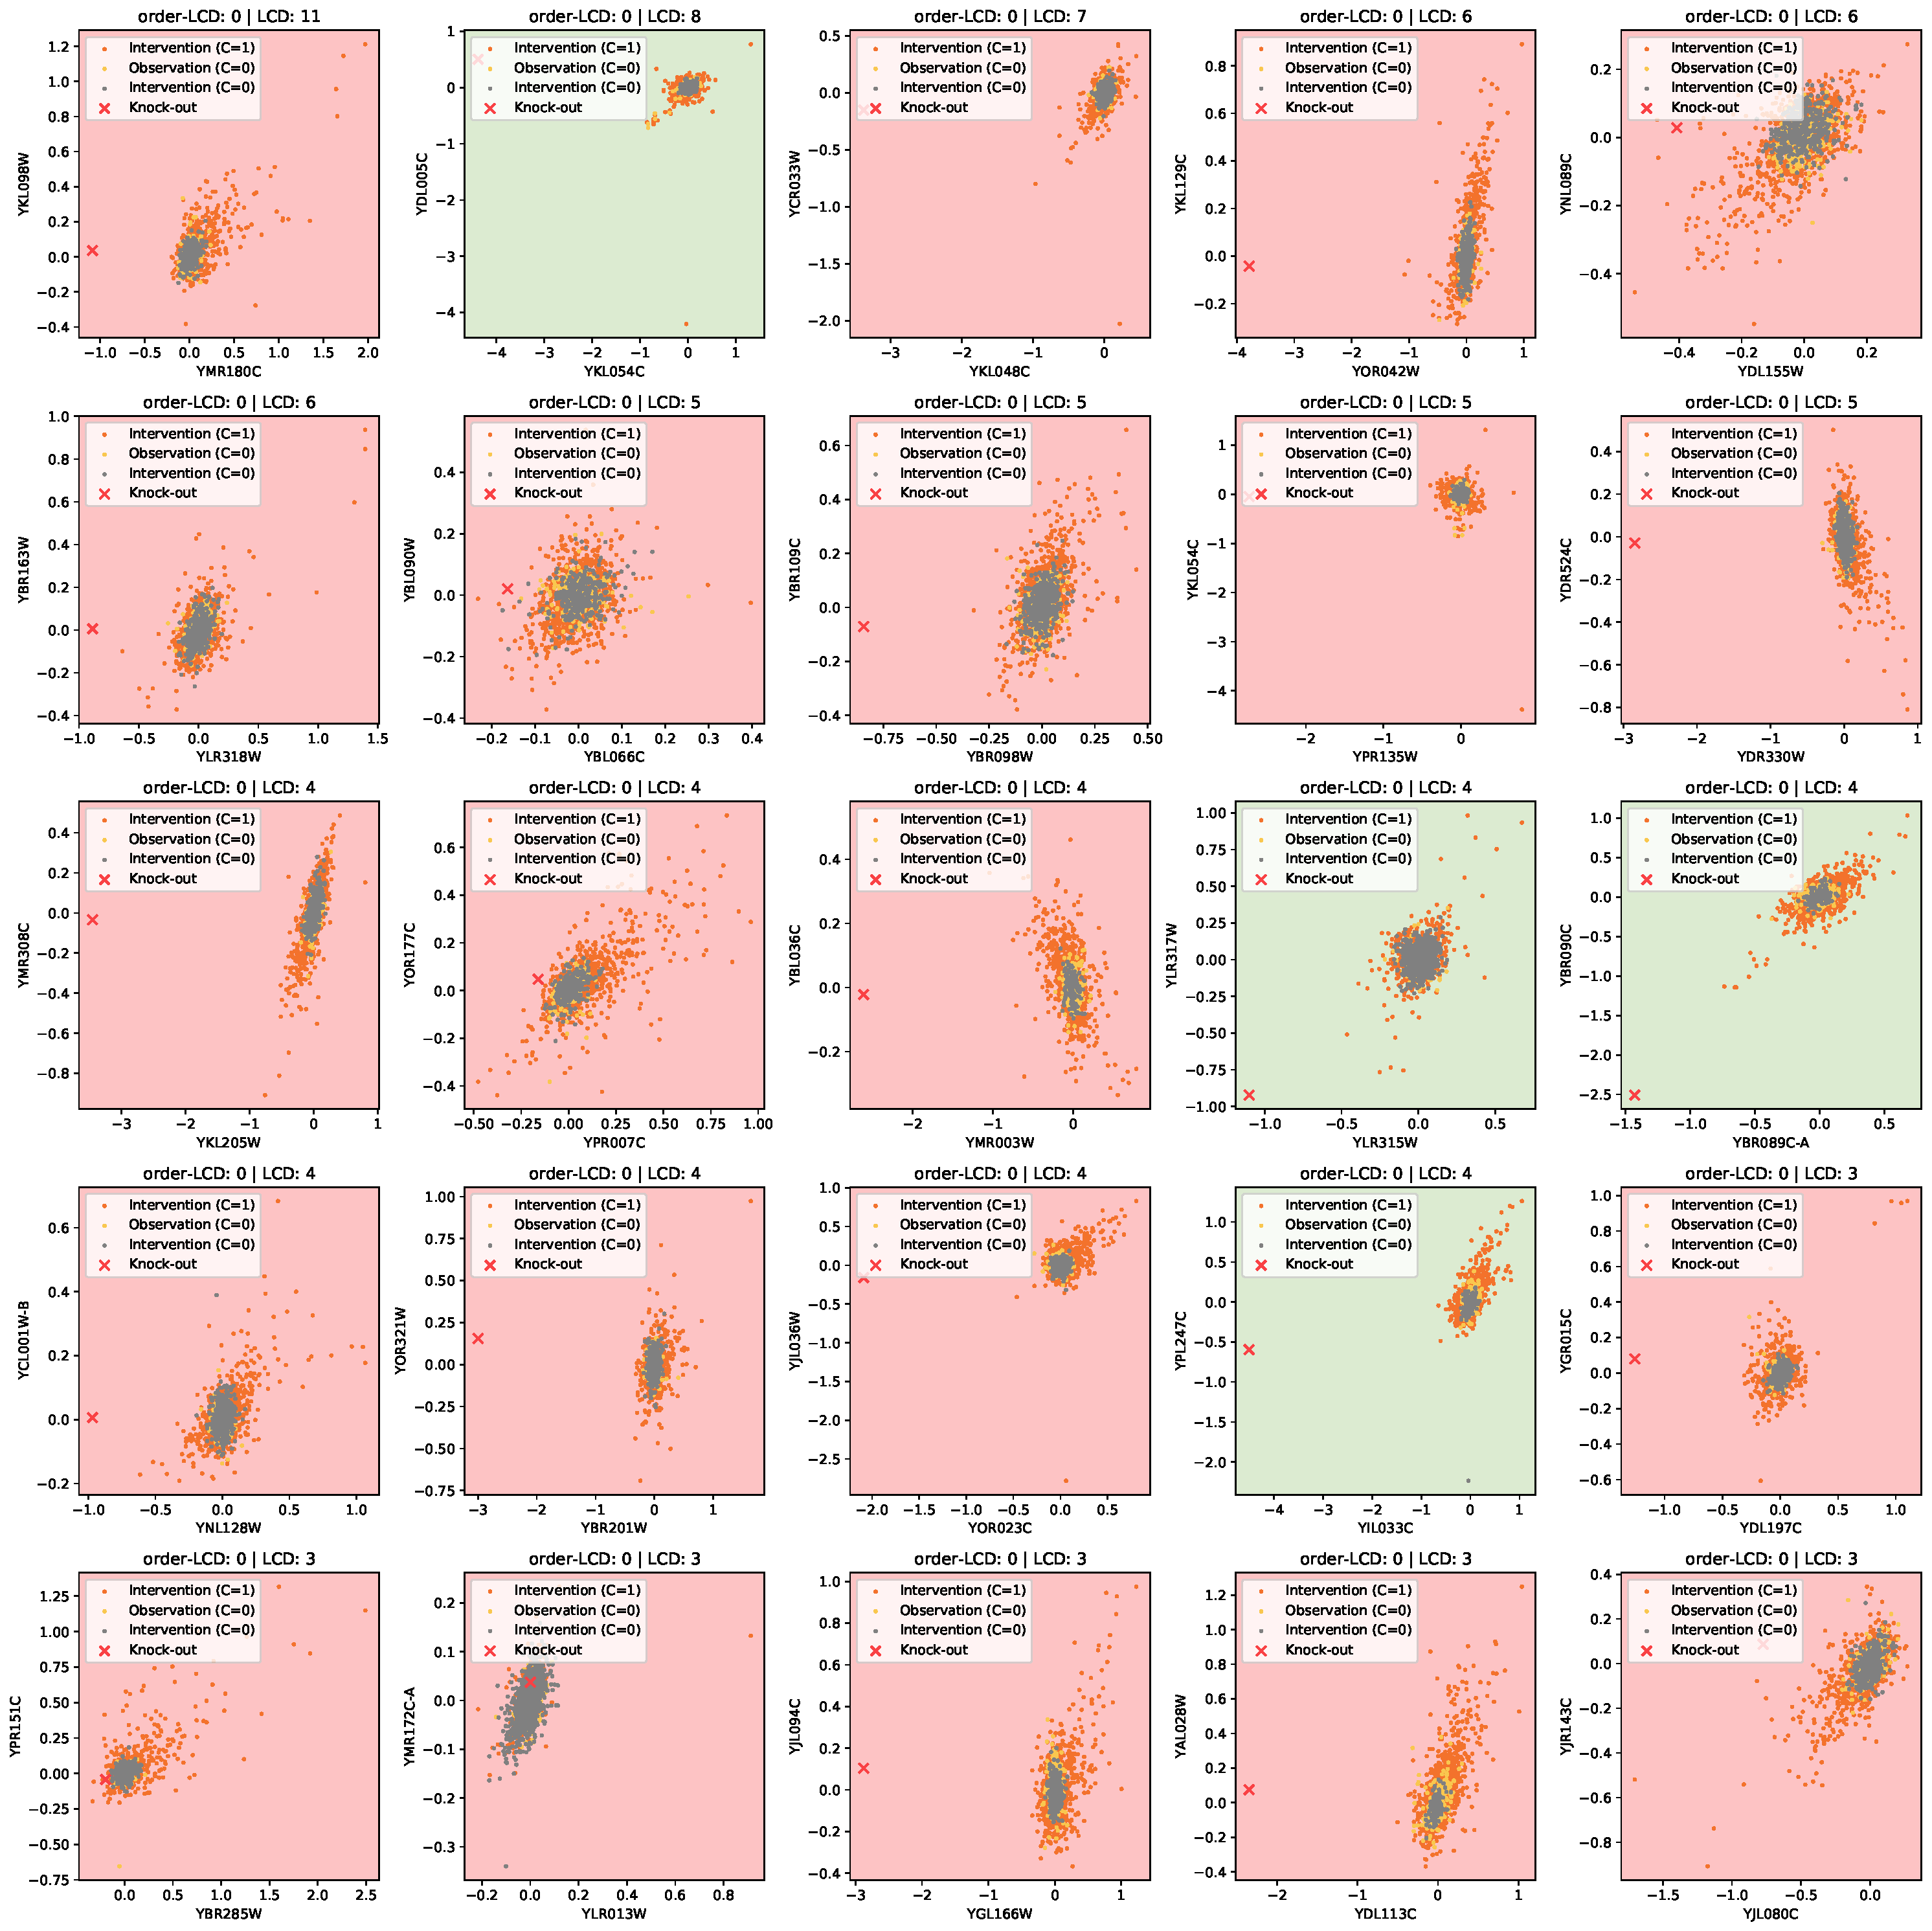
\includegraphics[width=\textwidth]{Bexclusive_lcd.pdf}
    \caption{The 25 strongest predictions by \textbf{LCD} that are also \textbf{excluded} in the order-based LCD predictions. The precise scores are shown above the figures. The background color indicates whether the relation is true according to the $10\%$ threshold.}
\end{figure}


\subsubsection{Expression Levels per Context Group}

% oLCD
\begin{figure}[H]
    \centering
    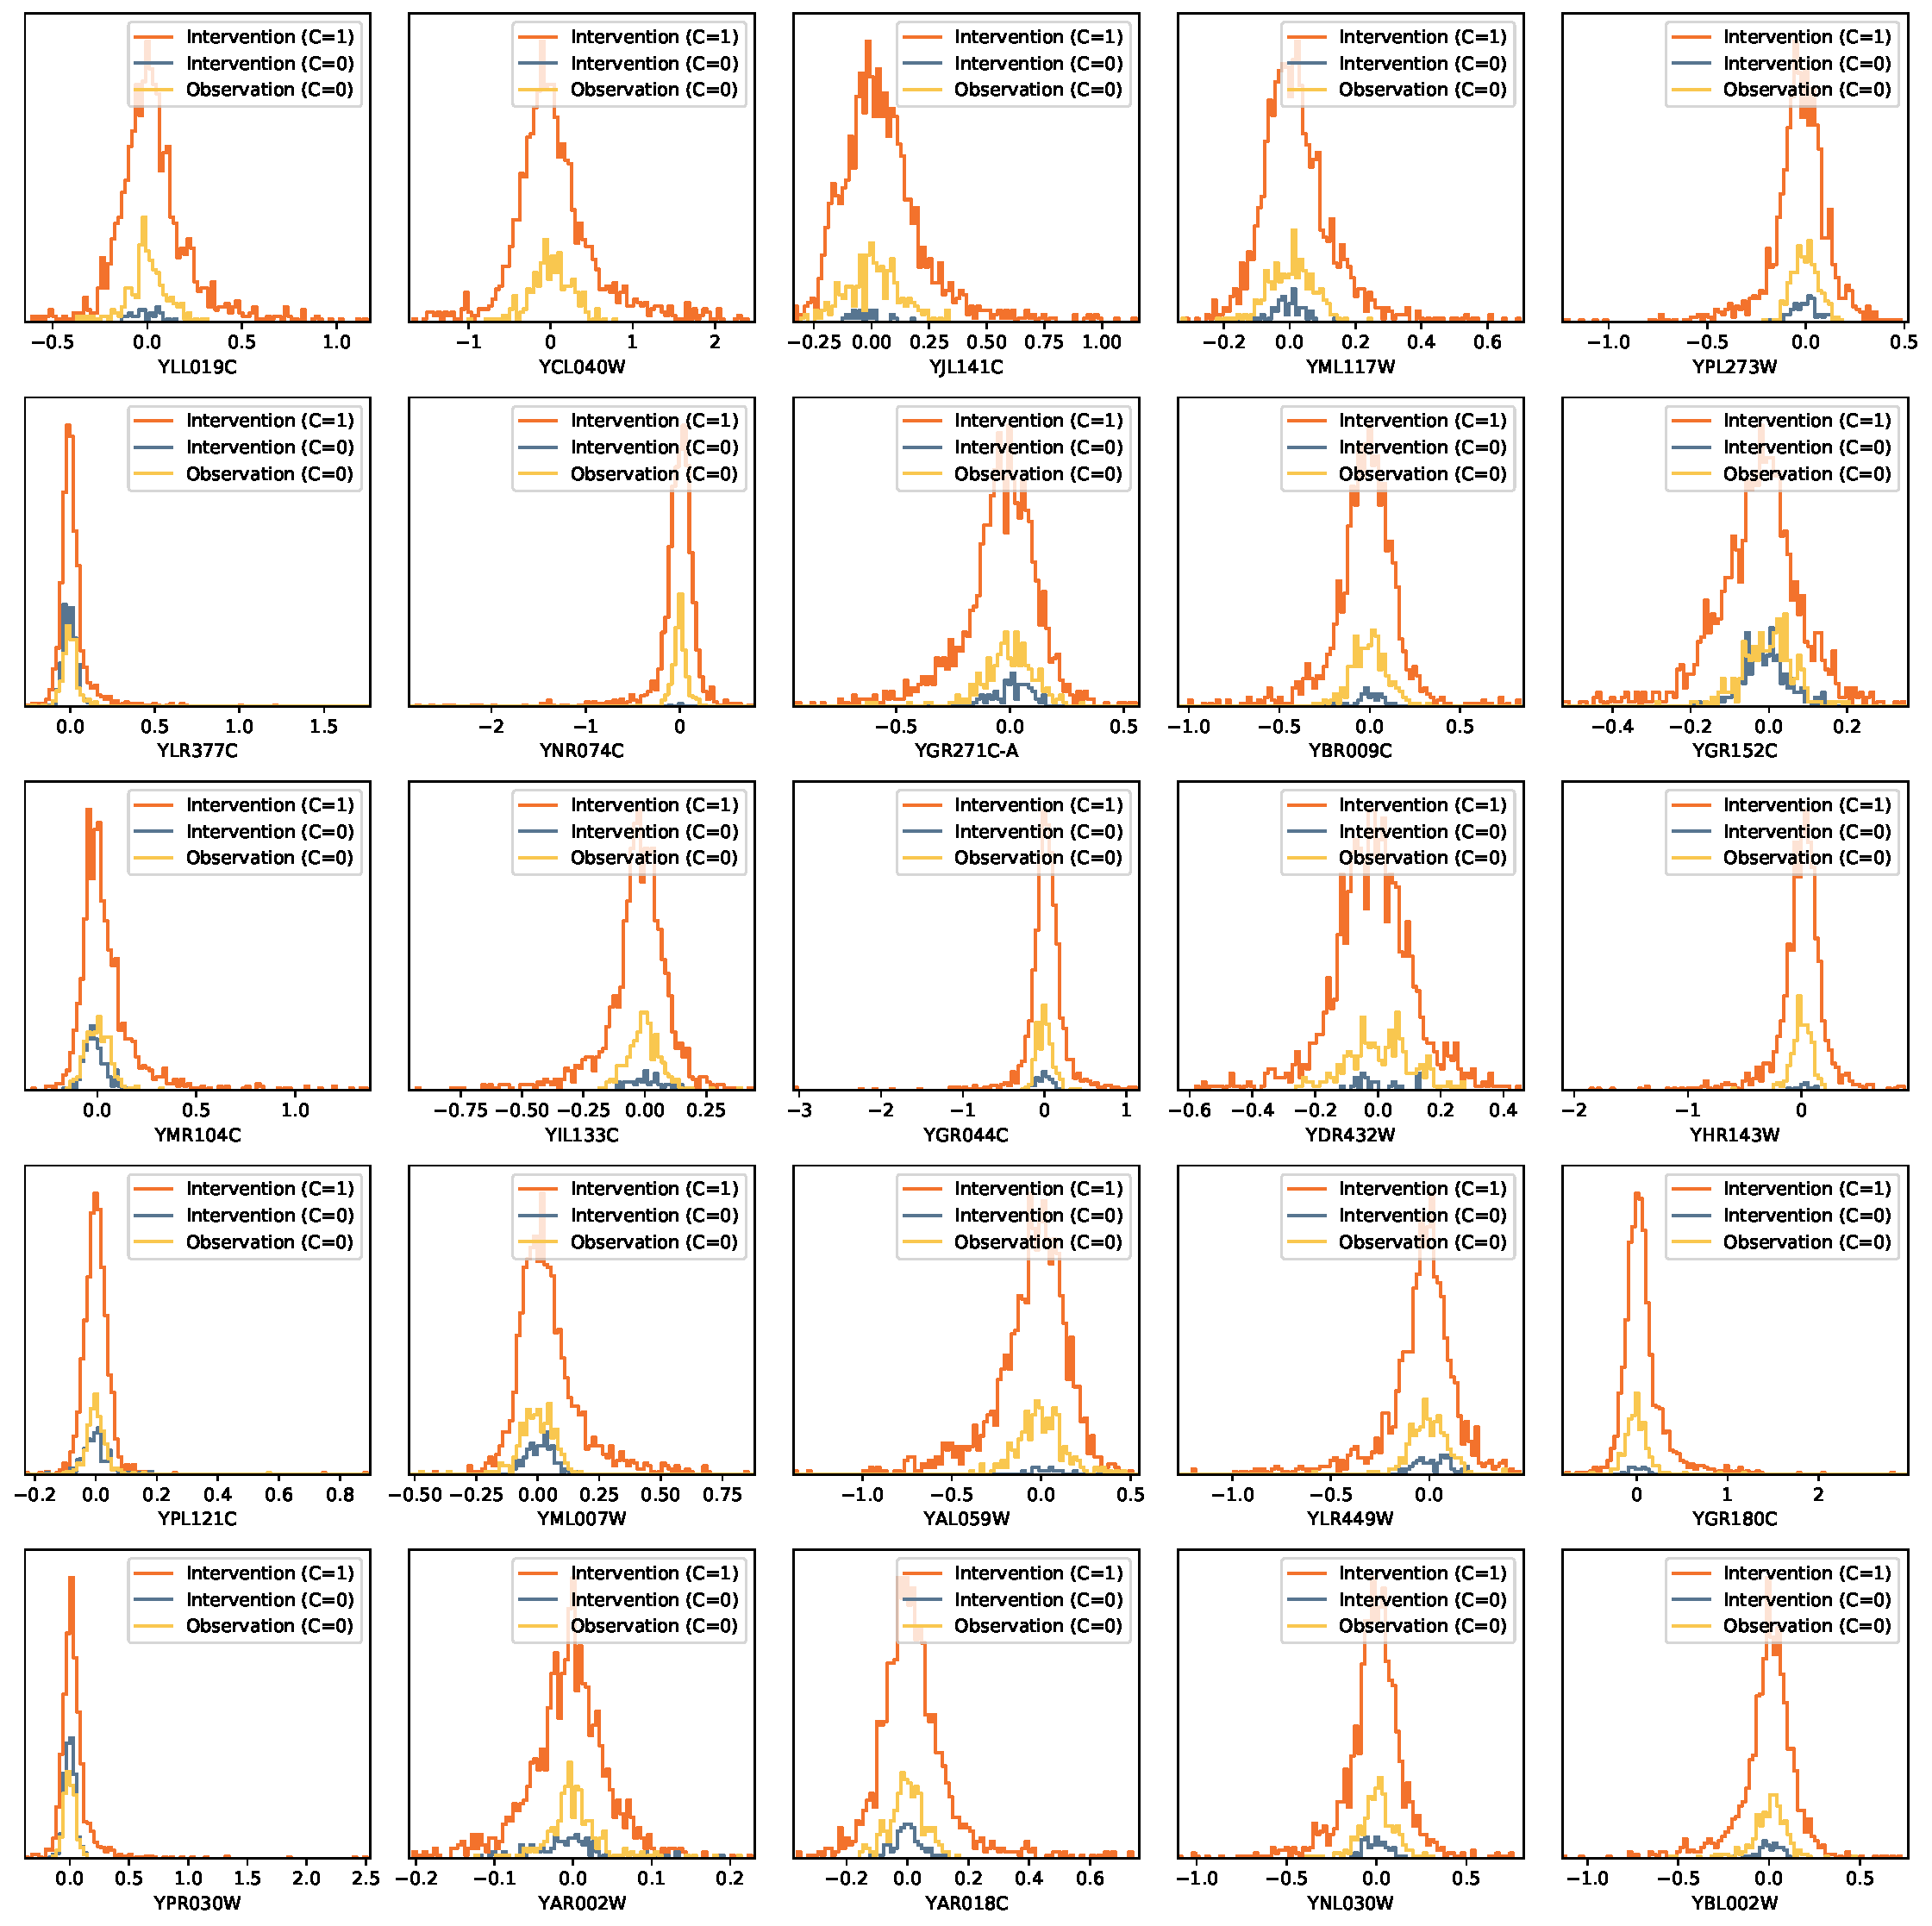
\includegraphics[width=\textwidth]{Bcontext_olcd.pdf}
    \caption{Distribution of the expression level of the cause genes in the strongest discrete predictions of \textbf{order-LCD}. Clusters are made based on whether the data points are observation or intervention data, and based on the context value if the data point is interventional.}
\end{figure}

% LCD
\begin{figure}[H]
    \centering
    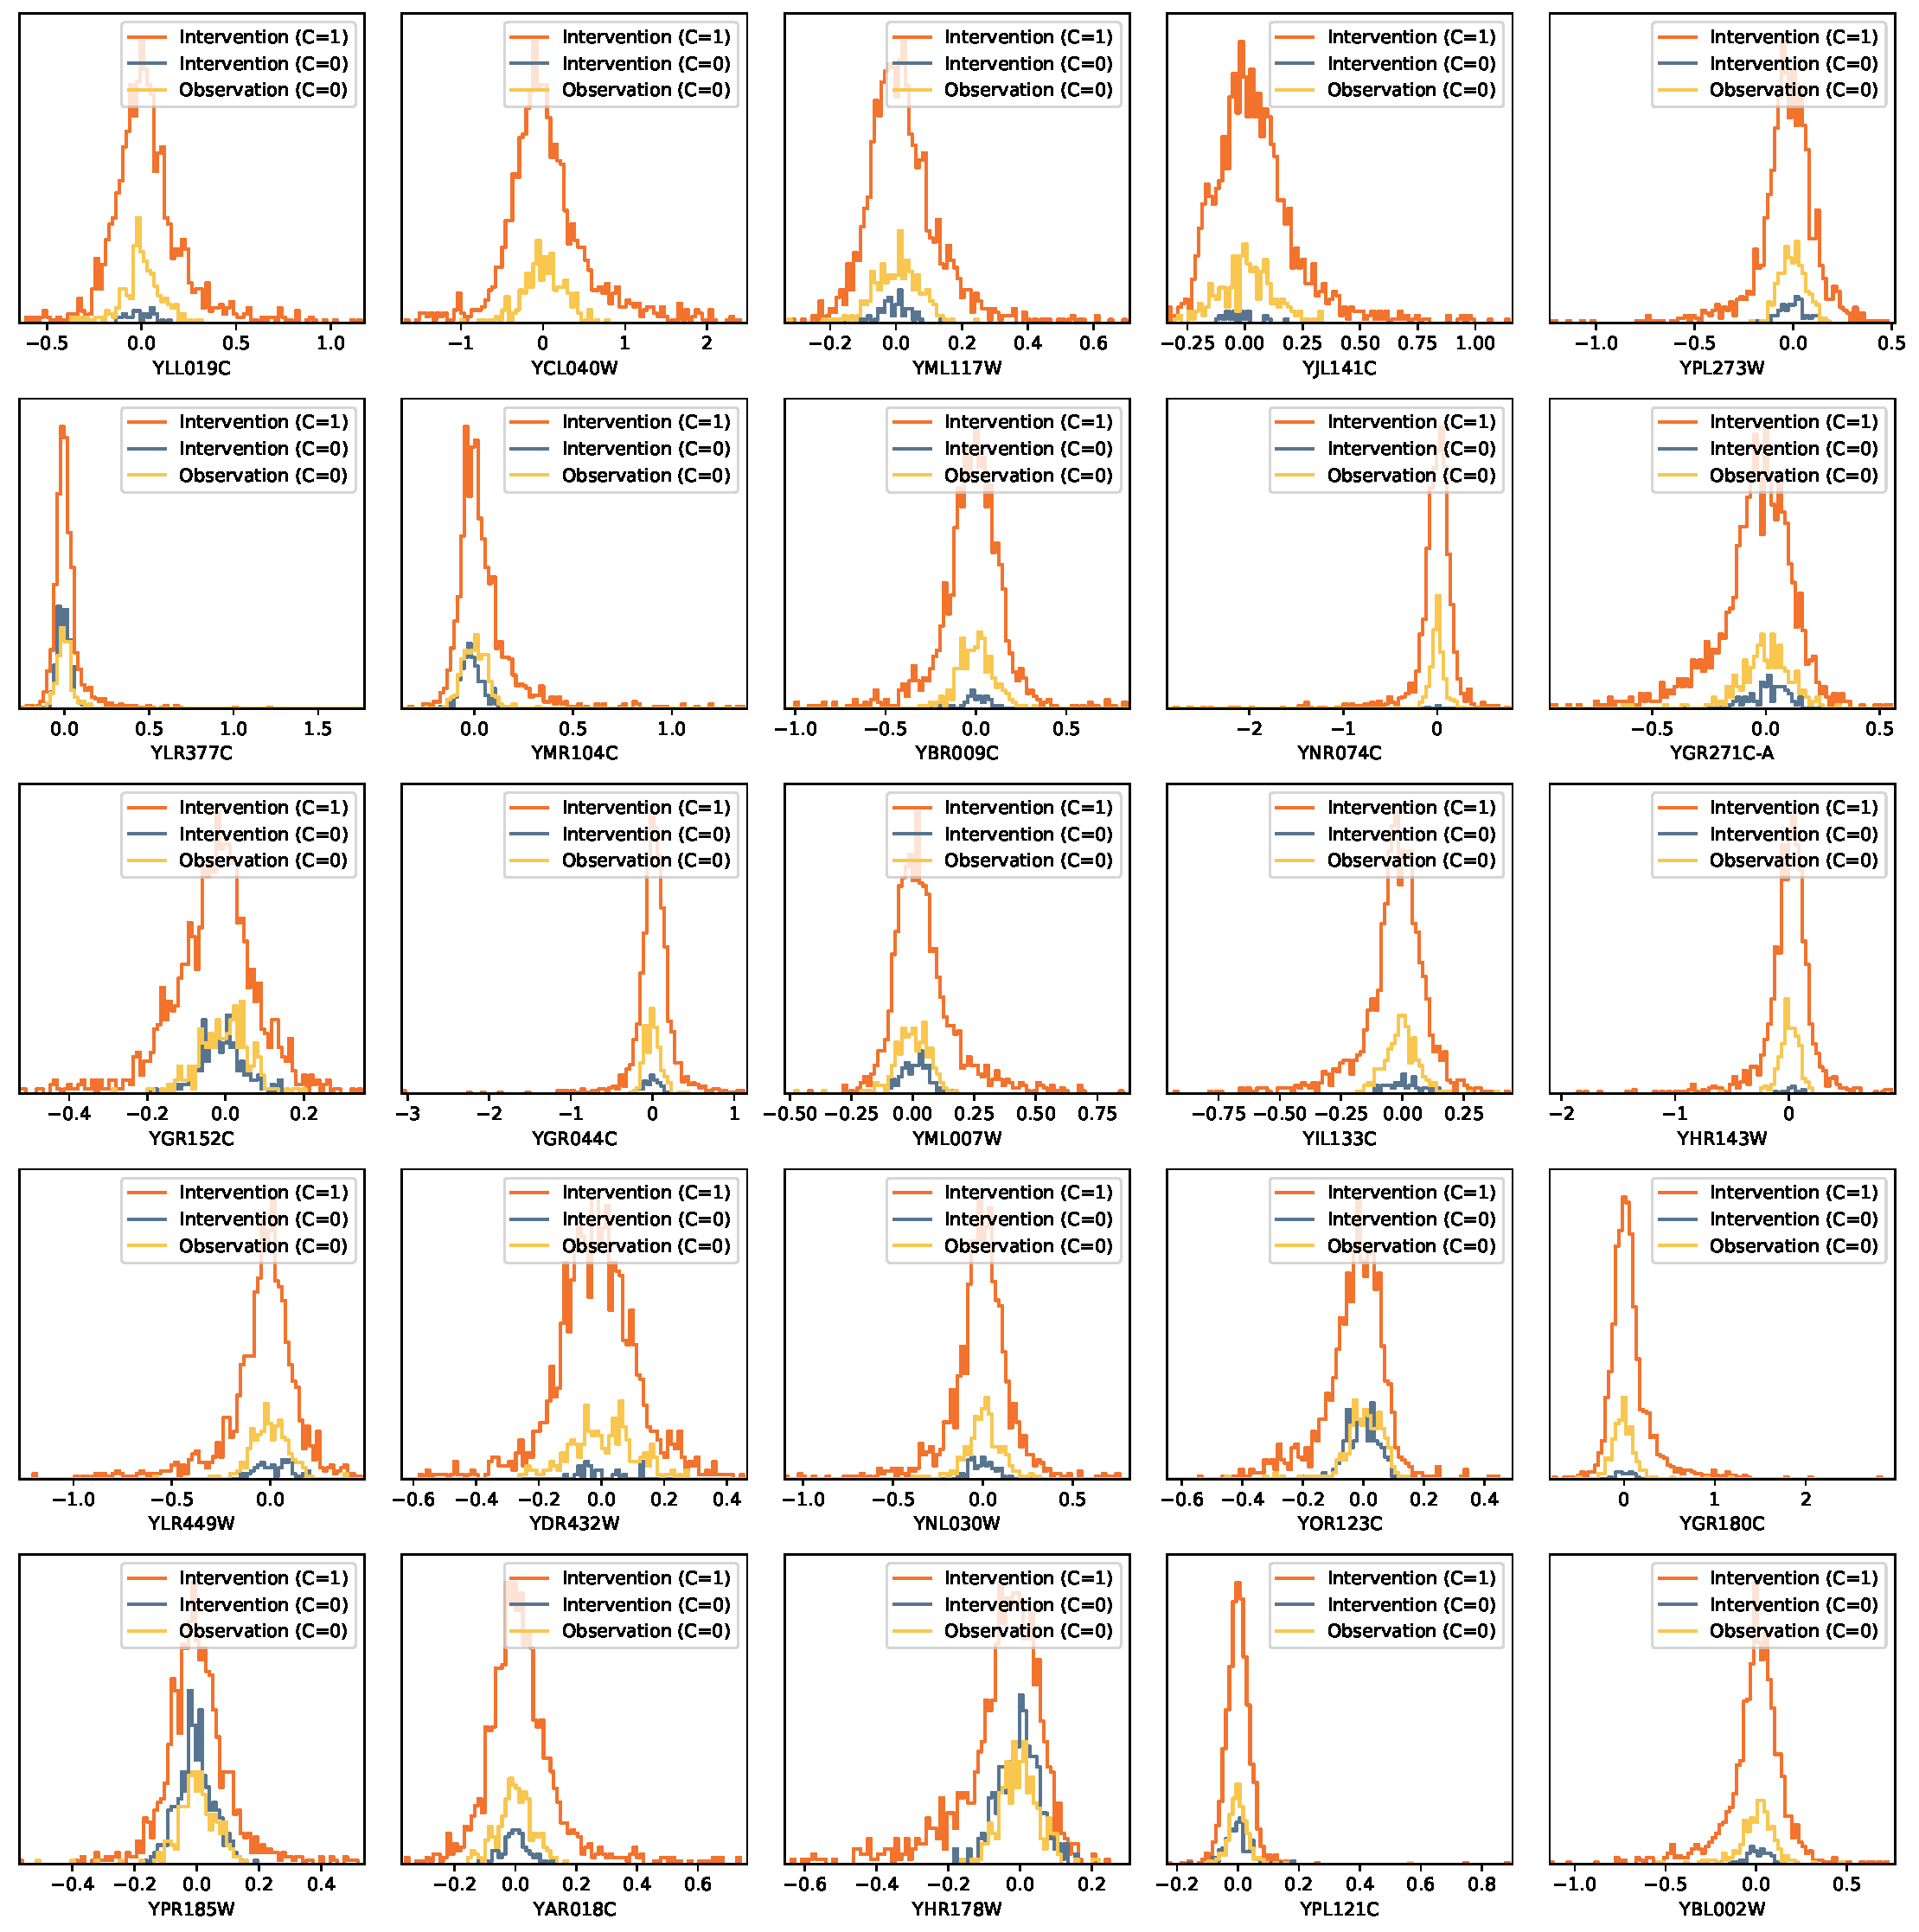
\includegraphics[width=\textwidth]{Bcontext_lcd.pdf}
    \caption{Distribution of the expression level of the cause genes in the strongest discrete predictions of the original \textbf{LCD}. Clusters are made based on whether the data points are observation or intervention data, and based on the context value if the data point is interventional.}
\end{figure}


% L2
\begin{figure}[H]
    \centering
    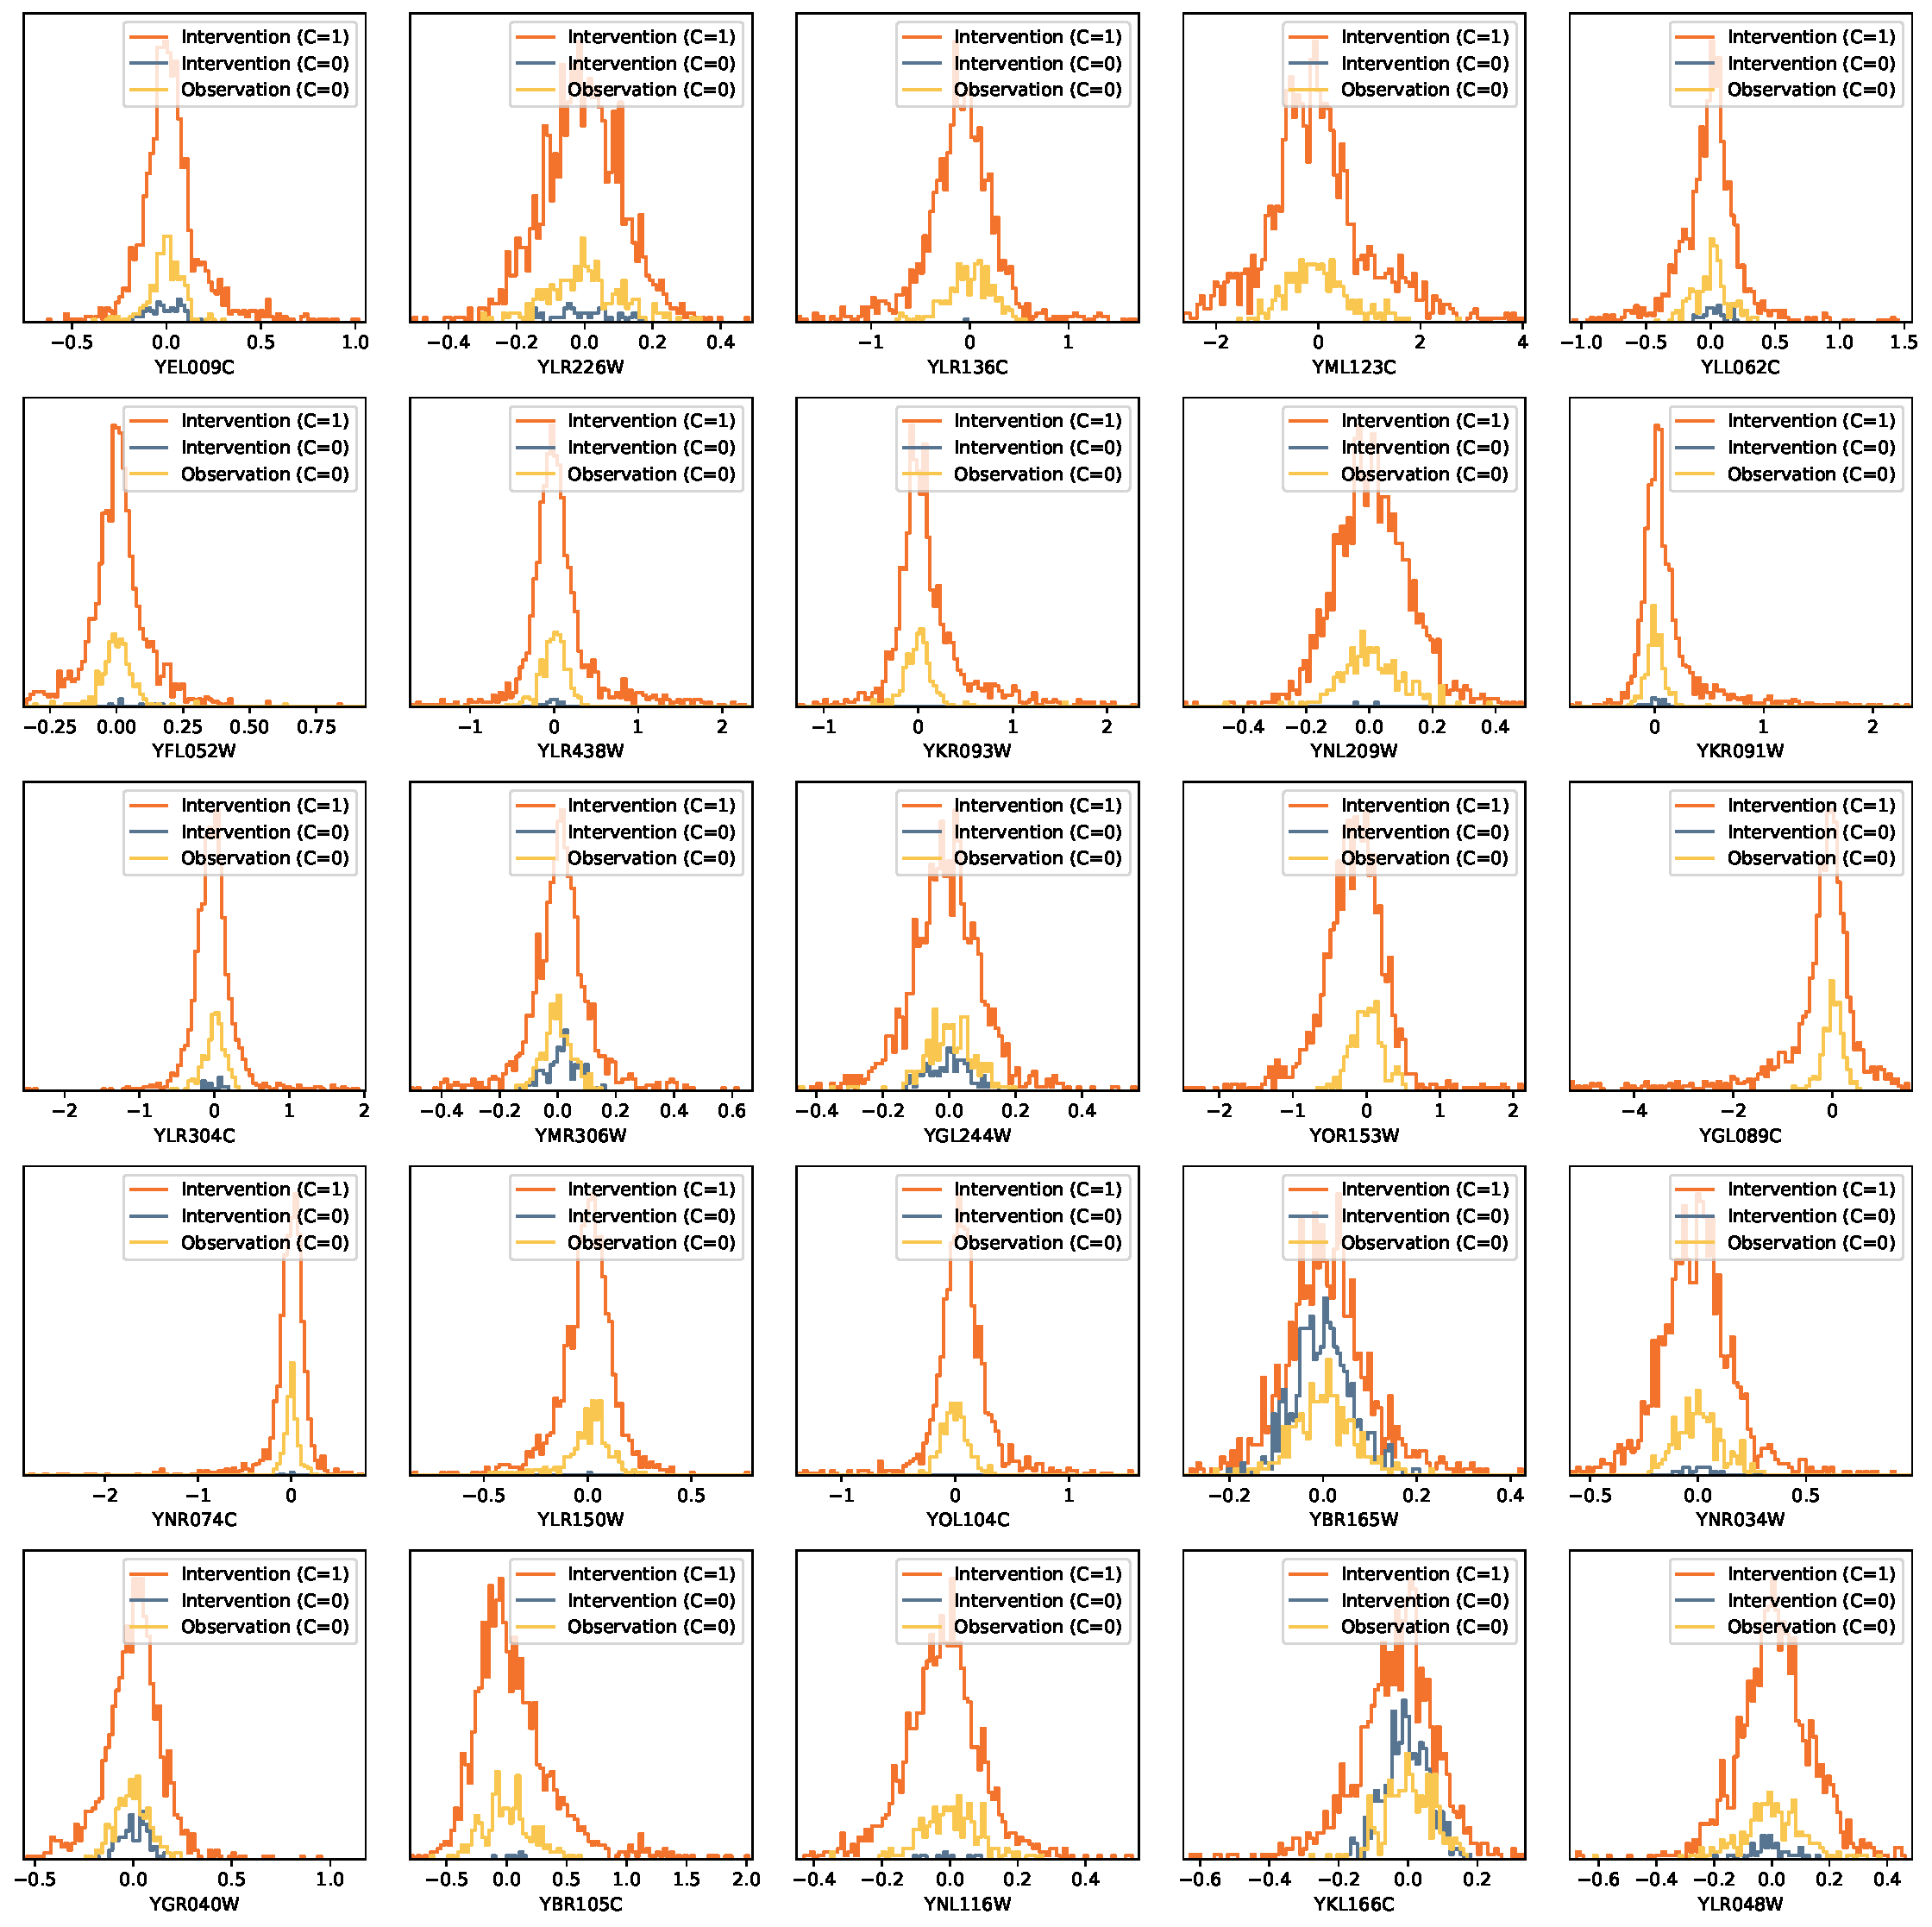
\includegraphics[width=\textwidth]{Bcontext_l2.pdf}
    \caption{Distribution of the expression level of the cause genes in the strongest discrete predictions of the \textbf{L$_2$-boosting baseline}. Clusters are made based on whether the data points are observation or intervention data, and based on the context value if the data point is interventional.}
\end{figure}

% random
\begin{figure}[H]
    \centering
    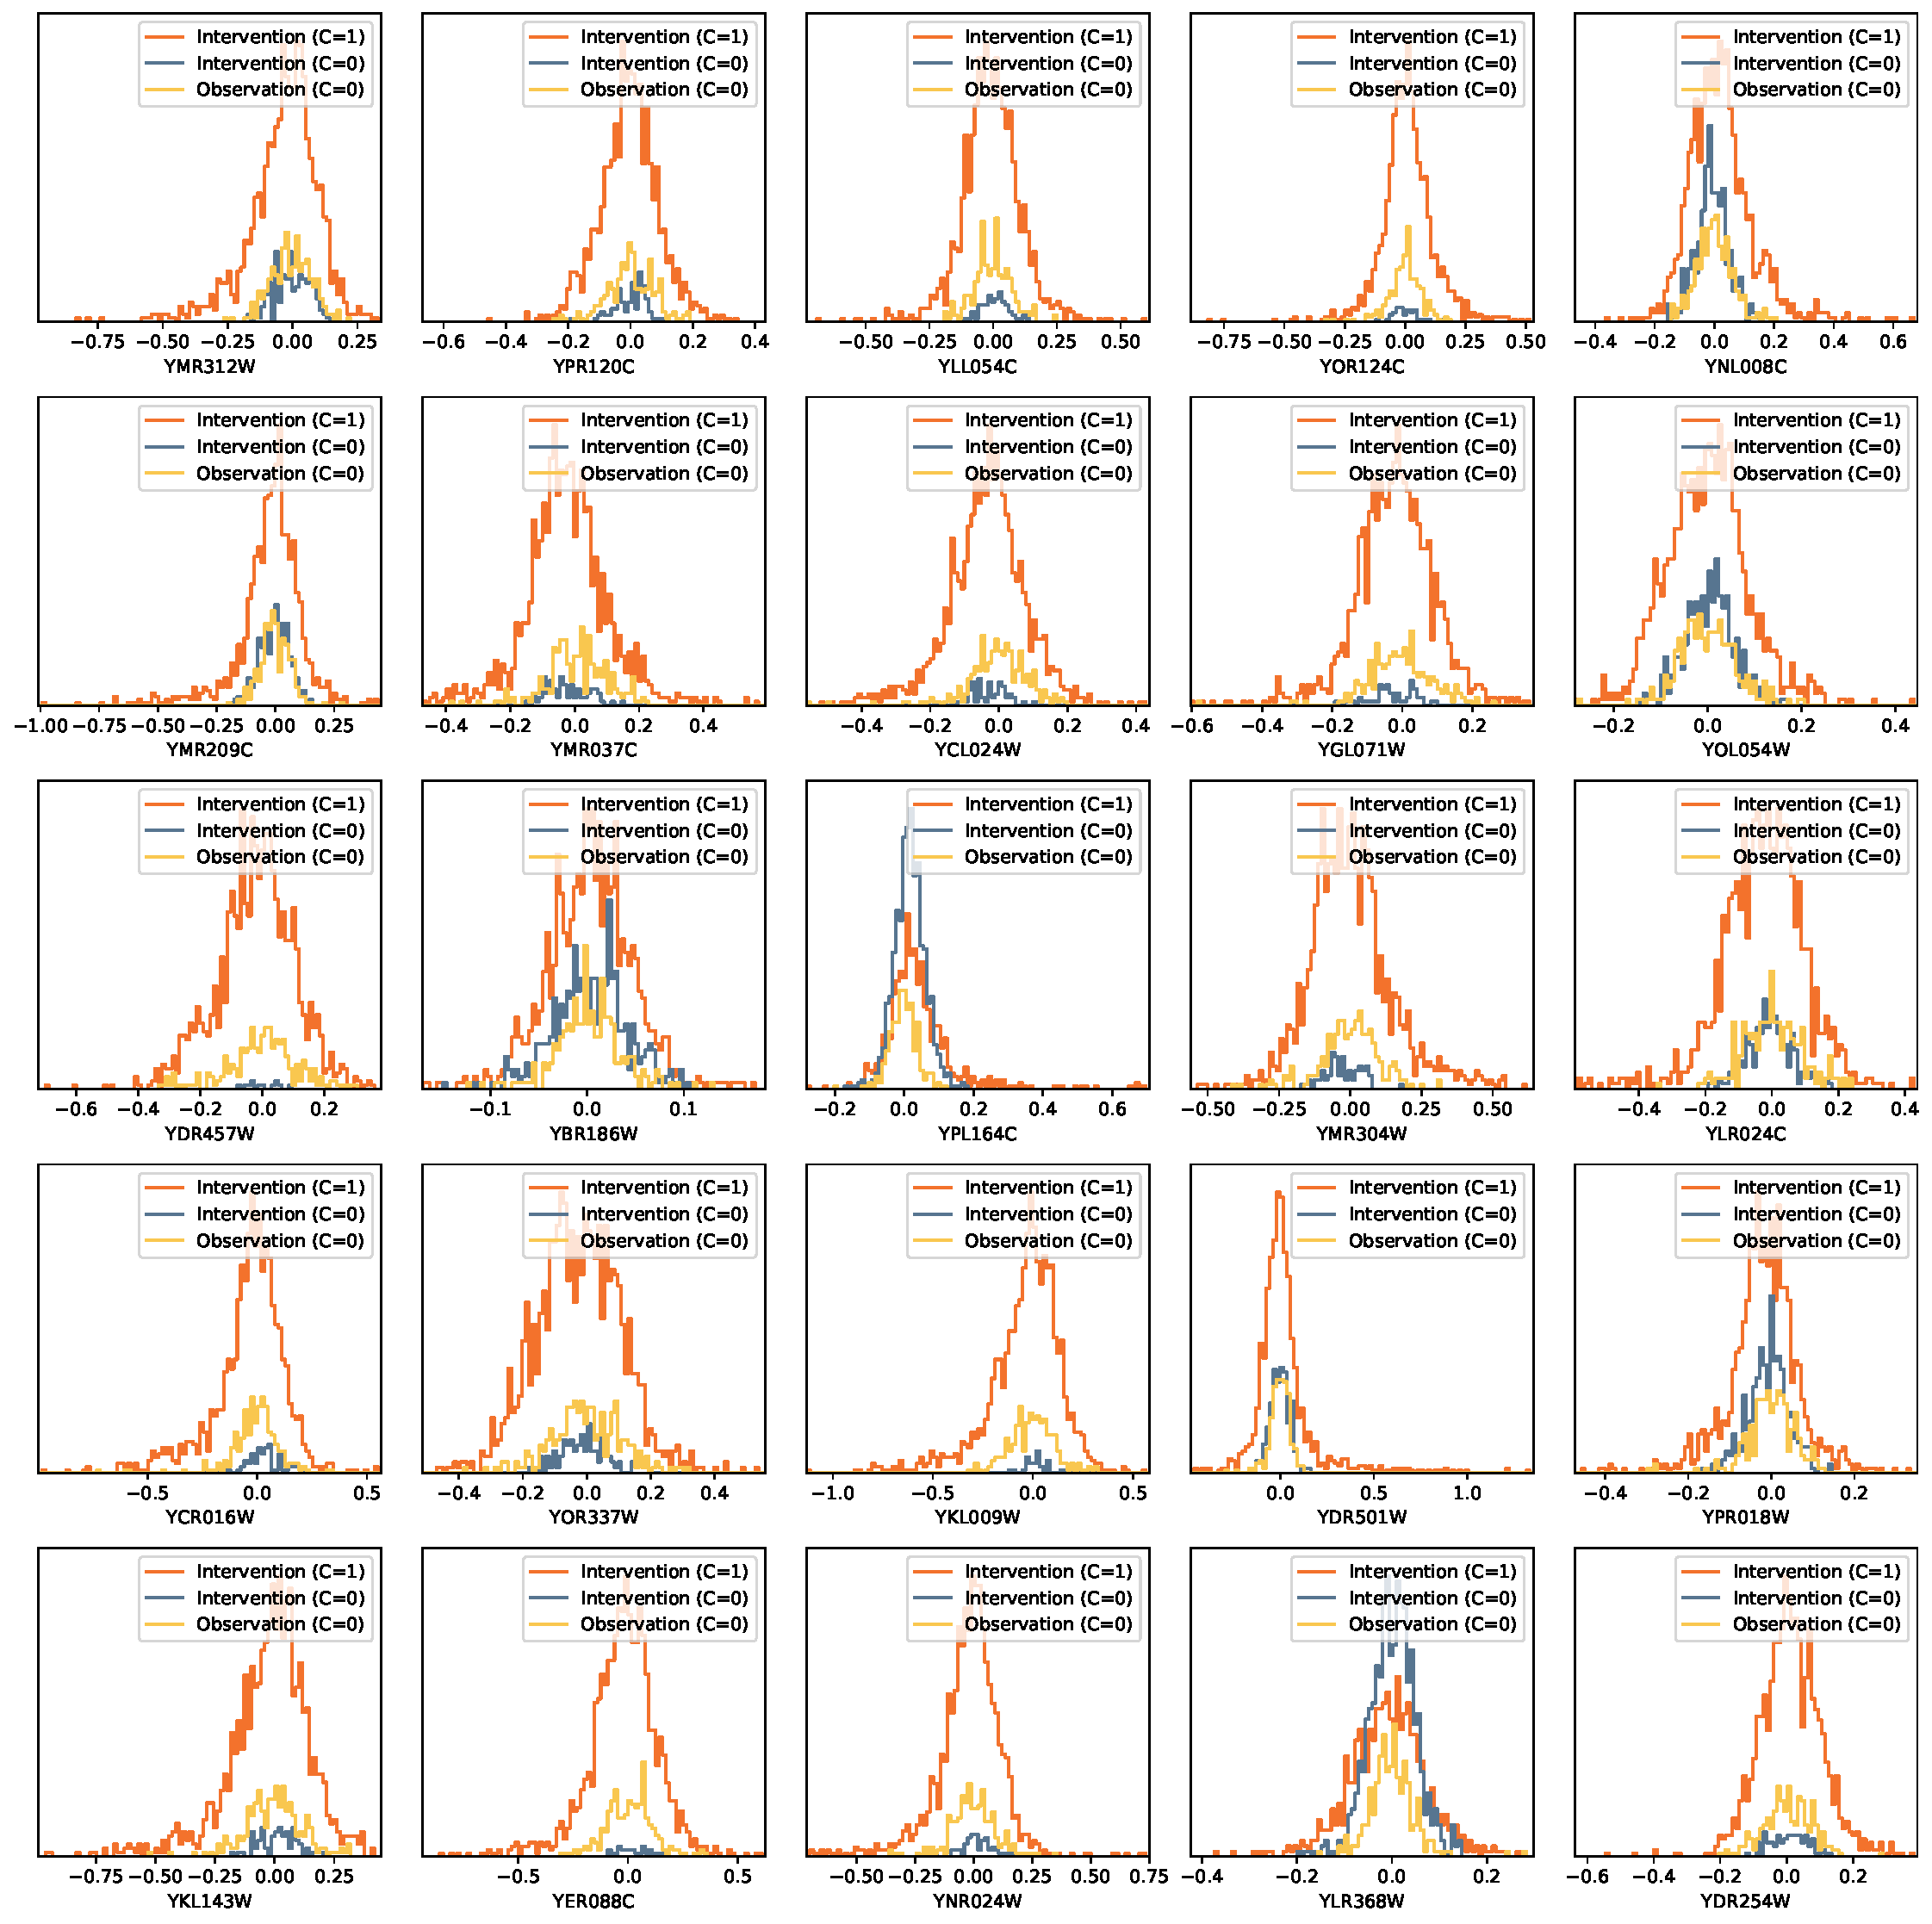
\includegraphics[width=\textwidth]{Bcontext_random.pdf}
    \caption{Distribution of the expression level of 25 \textbf{random} cause genes. Clusters are made based on whether the data points are observation or intervention data, and based on the context value if the data point is interventional.}
\end{figure}


% \newpage\phantom{blabla}